\documentclass[11pt]{article}
\usepackage[margin=1.1in]{geometry}
\usepackage{amsmath,amssymb,amsthm,mathtools,booktabs,graphicx,hyperref,natbib,algorithm,algpseudocode,caption,subcaption,microtype,xcolor,enumitem,longtable,array}
\newtheorem{theorem}{Theorem}
\newtheorem{proposition}[theorem]{Proposition}
\newtheorem{lemma}[theorem]{Lemma}
\newtheorem{corollary}[theorem]{Corollary}
\theoremstyle{definition}
\newtheorem{definition}[theorem]{Definition}
\newtheorem{example}[theorem]{Example}
\theoremstyle{remark}
\newtheorem{remark}[theorem]{Remark}
\newcommand{\todo}[1]{\textcolor{red}{[#1]}}
\bibliographystyle{plainnat}
\title{Certified Seat--Safety Frontiers for U.S.\ House Districting:\\ Counterexample-Guided Geographic Relaxation under County-Split Budgets}
\author{Draft}
\date{\today}
\begin{document}
\maketitle
\begin{abstract}
Heuristic algorithms can draw maps with many safe seats, but a map that has been found does not show that nothing better exists. We define the \emph{seat--safety frontier}, the largest number of U.S.\ House districts that can simultaneously clear a robust two-party margin $m$, and its dual, the \emph{spectrum} of best achievable $q$-th district margins, and we certify both at voting-precinct resolution. Our relaxations aggregate precincts into cells with exact-integer allocations, fractional-knapsack hull cuts and connectivity on the quotient graph; a counterexample-guided loop refines only the cells that a relaxed solution splits and ends with either an independently verified plan or an infeasibility proof. We prove that every relaxation is valid at atomic resolution, that refinement is monotone, and that a solution splitting no cell is an atomic plan. A negative result---provable on paths and visible on real precincts---shows that coarsening connectivity alone cannot beat the geography-free bound; a county-split budget, counted by pieces as in the exact county-split literature, is what makes coarse relaxations informative. For 16 states with two to five districts, both parties, 2020 precincts, $\pm1\%$ population balance and at most $k-1$ county splits, we bracket the spectrum to within half a point in 21 of 24 cases for the six two-district states (median width 2.2--2.6 points for states with three to five districts) and pin the number of districts reaching 50\%, 55\% and 60\% exactly in 79 of 96 cases. A subdivision budget matters in a certified way: each additional split raises the best-district share in Maine by about a point, and one extra split turns New Hampshire Republicans from zero to one district. Every bound is a verified map or an exact-integer proof, audited against an independent MILP encoding and against brute-force enumeration. The frontier is a capacity statement about district boundaries under a stated regime: it is symmetric in the parties, forecasts nothing and carries no legal claim.
\end{abstract}
\section{Introduction}\label{sec:intro}

How many congressional districts can a party make safe by drawing lines alone? Algorithms answer a weaker question. Given a vote map, a sampler or optimiser can \emph{find} a redistricting plan with many safe seats, but a plan that has been found says nothing about whether a better one exists: short-burst and column-generation methods are heuristics with no optimality guarantee \citep{cannon2023,gurnee2021,atlas2026}, and the exact integer programs that exist optimise compactness or county splits, not partisan outcomes \citep{validi2022,shahmizad2025}. The published dual bounds for representation objectives are for whole counties with a 10\% population tolerance \citep{fravel2026}, and coarsening the geography to make the optimisation easy \emph{restricts} the set of maps, so it yields a lower bound on what is possible, not an upper one. The consequence is that ``how many safe seats can the boundaries deliver?'' has, for real U.S.\ House geography, been answered only by lower bounds---and so has the question that follows from it, how far a given map is from what the boundaries allow.

This paper turns the question into a certification problem and answers it exactly at voting-precinct resolution for a class of realistic regimes. Our contributions are as follows.

\begin{enumerate}[leftmargin=*]
\item \textbf{A frontier and its dual.} We define the \emph{seat--safety frontier} $F(m)$---the largest number of districts that can simultaneously have a robust two-party share of at least $\tfrac12+m$---and the \emph{seat--safety spectrum} $\sigma^*(q)$, the largest achievable $q$-th best district margin. They are generalised inverses of each other (Theorem~\ref{thm:duality}), the area under $F$ is $\sum_q[\sigma^*(q)]_+$ (Corollary~\ref{cor:layer}), and both are monotone in the population tolerance, the subdivision budget and the scenario set (Proposition~\ref{prop:mono}). The single-threshold ``max seats'' objectives of earlier work are points on this curve, and at threshold $50\%$ the frontier of the two parties gives a certified \emph{seat range} for each state.
\item \textbf{Aggregated outer relaxations with a proof-carrying refinement loop.} We give a family of relaxations that aggregate precincts into cells, with exact-integer allocations, fractional-knapsack hull cuts and connectivity imposed on the quotient graph. We prove that every relaxation is valid at atomic resolution (Theorem~\ref{thm:valid}), that refinement is monotone (Theorem~\ref{thm:mono}), and that a solution splitting no cell \emph{is} an atomic plan (Theorem~\ref{thm:exact}). A counterexample-guided loop refines only the cells that a relaxed solution splits and ends with either an independently verified plan or an infeasibility proof (Theorem~\ref{thm:cegar}).
\item \textbf{A negative result and a fix.} Coarsening connectivity alone is provably (Proposition~\ref{prop:blind}) and empirically (Section~\ref{sec:negative}) unable to improve on the geography-free bound until cells are almost single precincts. A subdivision budget, counted in county splits as in the exact county-split literature, confines the looseness to a few counties at every refinement level (Proposition~\ref{prop:confine}) and makes the loop terminate quickly.
\item \textbf{Certified frontiers for real states.} For 16 states with two to five districts and both parties, using 2020 precincts, $\pm1\%$ population balance and at most $k-1$ county splits, we bracket the whole spectrum: 44 of 104 brackets are tight to half a point (median width 0.01 point in the six two-district states, 2.2--2.6 points for $3\le k\le5$), and the number of districts that can reach 50\%, 55\% and 60\% of the two-party vote is pinned exactly in 79 of 96 (state, party, threshold) cases (Section~\ref{sec:results}). Every bound is either an independently verified map or an exact-integer infeasibility proof, audited against a second solver and against brute-force enumeration; on the 20 queries that produce the upper ends of the two-district brackets the loop decides all, while exact solvers on the atomic model leave 6 (CP-SAT) or 7 (HiGHS) undecided after 300 s (Section~\ref{sec:baseline}).
\item \textbf{Seat ranges and a yardstick for enacted maps.} Across the 52 seats of these states, verified plans of the regime attain total counts of Democratic-majority districts (2020 presidential vote) from $11$ to $30$, and the proofs exclude anything outside $11$--$36$; Iowa, Nevada and New Mexico are states in which each party can draw a majority of the delegation, while in four states the delegation is the same for every plan. Rendered at precinct resolution, no enacted 118th-Congress plan reaches the certified capacity at any rank (median shortfall 5.9 points of district share), and the eight enacted plans that satisfy the regime give an independent, non-algorithmic test of the proofs, which none violates (Section~\ref{sec:enacted}).
\item \textbf{Budget, tolerance and scenarios.} Each extra county split provably raises Maine's best-district capacity by roughly a point (and turns New Hampshire Republicans from zero to one district), the population tolerance matters by at most half a point, and requiring a margin to hold across all statewide contests can cut a party's capacity by nearly ten points, so the spectrum doubles as a durability measure. The certified brackets and witness plans also serve as ground truth for scoring heuristic optimisers, which in our runs fall one to two points short in the largest cases.
\end{enumerate}

\paragraph{What this is not.} The frontier is a statement about the \emph{capacity of boundaries} given a vote geography and an explicitly stated regime. It is symmetric in the parties, is not a forecast, recommends no map, and makes no legal claim: satisfying our regime is neither necessary nor sufficient for a plan to be lawful, enacted plans were drawn under criteria our model does not include, and regimes with additional legal constraints are sub-regimes whose frontiers are, by monotonicity, bounded above by ours.

\section{Related work}\label{sec:related}

\paragraph{Heuristic extremal maps and ensembles.}
Most computational work on extreme partisan maps is heuristic. Recombination and sequential Monte Carlo samplers \citep{deford2021,mccartan2023} generate ensembles; short-burst hill climbing \citep{cannon2023} and column generation \citep{gurnee2021} optimise chosen objectives; multilevel schemes \citep{swamy2023} approximate Pareto fronts; Ising-model and integer-programming-plus-local-search heuristics target maximally tilted assignments \citep{okamoto2021} and majority-minority districts \citep{brous2025}, and a mixed-integer model combines district drawing with targeted campaigning \citep{deshpande2023}; and recent studies map how large the achievable partisan swings are \citep{goedert2024} and how durable optimised majorities are under electoral change \citep{palmer2026}. The public Algorithmic Redistricting Atlas publishes short-burst ``Max'' (51\%) and ``Safe Max'' (55\%) maps and states explicitly that they carry no optimality guarantee \citep{atlas2026}. Ensemble analyses place enacted plans within a neutral baseline (for New Hampshire, \citealp{mcwhorter2026}); Section~\ref{sec:enacted} places them instead relative to certified extremes. These methods produce feasible plans---lower bounds on our frontier---but not proofs that nothing better exists. We use a county-aware recombination hill climber only as a source of verified incumbents.

\paragraph{Exact integer programming for districting.}
Integer programming for districting goes back to \citet{hess1965}. The key modelling advance is exact contiguity: \citet{validi2022} give branch-and-cut formulations with lazily separated connectivity cuts, \citet{miyazawa2021} study formulations for balanced connected partitions, and \citet{jolly2026} catalogue \emph{inexact} contiguity constraints that can exclude valid maps---which would invalidate any claimed upper bound. \citet{shahmizad2025} compute the exact minimum number of county splits for every state. Those works optimise compactness or splits; none optimises a partisan seat-count objective with a proof.

\paragraph{Bounds for representation objectives.}
Two lines are close to ours. \citet{duchin2019} derive rigorous \emph{geography-free} infeasibility bounds for the number of districts a party can win in Massachusetts by sorting towns or precincts by partisan margin per capita (with a pseudo-polynomial knapsack dynamic programme where sorting is inconclusive), for districts built from arbitrary collections of units without any spatial requirement; our geography-free baseline (Section~\ref{sec:negative}) is the same idea extended to the whole margin spectrum and to $k$-way allocations, in the spirit of the theory of optimal gerrymandering with unconstrained geography \citep{owen1988,friedman2008}, which is also studied as an optimisation problem in its own right \citep{benade2021} and, with uncertainty about district-level outcomes, in a stylised continuous model \citep{lagarde2024}. On the theory side, maximising the seats of a party is NP-complete on planar graphs and admits constant-factor approximations there \citep{dippel2024}; our exact and certified results are computational, for the graphs that arise from real precincts. \citet{fravel2026} prove dual bounds for non-convex expected-representation objectives with exact contiguity, but for whole-county instances only, with a 10\% population tolerance and at most seven districts. Because forcing counties whole \emph{restricts} the plan class, a county-level optimum is not an upper bound for maps with finer resolution; the relaxations of Section~\ref{sec:relax} are valid at precinct resolution by construction.

\paragraph{Adaptive refinement.}
Our algorithm is an instance of counterexample-guided abstraction refinement \citep{clarke2003} and is analogous to dynamic discretization discovery in transportation \citep{boland2017,marshall2021}: solve a small relaxation whose optimum is a valid bound, refine only where the relaxed solution is spurious, and stop when the answer is proved or an exact solution appears. What is specific to districting is the abstraction: cells with exact-integer aggregate allocations, fractional-knapsack hull cuts and quotient-graph connectivity, together with a subdivision budget that makes coarse abstractions informative.

% ---------------------------------------------------------------------------
\section{The seat--safety frontier and spectrum}\label{sec:frontier}

\paragraph{Instances.}
An \emph{instance} consists of a connected graph $G=(V,E)$ of \emph{atoms} (in our application: 2020 voting precincts, adjacent when they share boundary), a partition $\mathcal K$ of $V$ into \emph{subdivisions} (counties), integer populations $p_i\ge 0$, a finite set $\Omega$ of \emph{scenarios} (statewide contests), integer two-party vote counts $D_{i\omega},R_{i\omega}\ge 0$, and a number of districts $k$. For $A\subseteq V$ write $p(A)=\sum_{i\in A}p_i$ and $T=p(V)$. For a party $\pi\in\{D,R\}$ let $P_{i\omega}$ be its votes and $O_{i\omega}$ the other party's votes.

\paragraph{Plans and regimes.}
A \emph{regime} is a triple $\rho=(\varepsilon,s,\Omega)$: a population tolerance $\varepsilon\ge0$, a \emph{subdivision budget} $s\in\{0,1,\dots\}\cup\{\infty\}$, and a scenario set. Let $L=\lceil(1-\varepsilon)T/k\rceil$ and $U=\lfloor(1+\varepsilon)T/k\rfloor$. A \emph{plan} is a partition $M=\{V_1,\dots,V_k\}$ of $V$ into $k$ nonempty parts. It is \emph{$\rho$-feasible} if
\begin{enumerate}
\item[(a)] every $G[V_j]$ is connected;
\item[(b)] $L\le p(V_j)\le U$ for all $j$;
\item[(c)] at most $s$ splits, where $\mathrm{split}(M)=\sum_{K\in\mathcal K}\bigl(d_K(M)-1\bigr)$ and $d_K(M)\ge1$ is the number of parts meeting $K$: a subdivision divided among $d$ districts counts $d-1$ splits, as in the county-split literature \citep{shahmizad2025}.
\end{enumerate}
Let $\mathcal M_\rho$ be the set of $\rho$-feasible plans. The regime is a \emph{modelling} choice: satisfying it is neither necessary nor sufficient for legality, and the paper makes no legal claim.

\paragraph{Robust margins.}
The \emph{robust margin} of a district $V_j$ for party $\pi$ is
\[
r^\pi_j(M)=\min_{\omega\in\Omega}\Bigl(\frac{P_\omega(V_j)}{P_\omega(V_j)+O_\omega(V_j)}-\frac12\Bigr),
\]
where $P_\omega(A)=\sum_{i\in A}P_{i\omega}$ (all instances used here have positive vote totals in every plausible district). Sorting the margins of a plan in decreasing order gives $r^\pi_{(1)}(M)\ge\dots\ge r^\pi_{(k)}(M)$.

\begin{definition}[Frontier and spectrum]
For $m\ge0$ and $q\in\{1,\dots,k\}$,
\[
F^\pi_\rho(m)=\max_{M\in\mathcal M_\rho}\bigl|\{j:\ r^\pi_j(M)\ge m\}\bigr|,
\qquad
\sigma^{*,\pi}_\rho(q)=\max_{M\in\mathcal M_\rho} r^\pi_{(q)}(M),
\]
(both defined when $\mathcal M_\rho\neq\emptyset$). $F$ is the \emph{seat--safety frontier}: the largest number of districts that can simultaneously win with a robust cushion of $m$ share points over one half. $\Sigma^*=(\sigma^*(1),\dots,\sigma^*(k))$ is the \emph{seat--safety spectrum}.
\end{definition}

The frontier generalises the single-threshold objectives of heuristic ``maximum'' maps (for instance the 51\% and 55\% maps of the Algorithmic Redistricting Atlas \citep{atlas2026}) to a whole curve, and $m=0$ recovers the largest feasible number of majority districts.

\needspace{12\baselineskip}
\begin{proposition}[Monotonicity and symmetry]\label{prop:mono}
Fix an instance and party.
\begin{enumerate}
\item $m\mapsto F_\rho(m)$ is non-increasing; $q\mapsto\sigma^*_\rho(q)$ is non-increasing.
\item If $\Omega\subseteq\Omega'$ then $F_{(\varepsilon,s,\Omega)}\ge F_{(\varepsilon,s,\Omega')}$ pointwise.
\item If $\varepsilon\le\varepsilon'$ and $s\le s'$ then $\mathcal M_{(\varepsilon,s,\Omega)}\subseteq\mathcal M_{(\varepsilon',s',\Omega)}$, hence $F_{(\varepsilon,s,\Omega)}\le F_{(\varepsilon',s',\Omega)}$ and $\sigma^*$ likewise.
\item Swapping the roles of the two parties in all vote data maps $F^D$ to $F^R$ (and $\sigma^{*,D}$ to $\sigma^{*,R}$) exactly.
\end{enumerate}
\end{proposition}
\begin{proof}
(1)--(3) are immediate from the definitions (a smaller scenario set lowers a minimum; a larger regime enlarges the feasible set). (4): the margins are computed from $(P,O)$, which the swap exchanges.
\end{proof}

\begin{theorem}[Spectrum duality]\label{thm:duality}
If $\mathcal M_\rho\neq\emptyset$ then for all $m$ and $q$: $F_\rho(m)\ge q\iff\sigma^*_\rho(q)\ge m$. Consequently $F_\rho(m)=\max\{q:\sigma^*_\rho(q)\ge m\}$ (with $\max\emptyset=0$) and $\sigma^*_\rho(q)=\max\{m: F_\rho(m)\ge q\}$.
\end{theorem}
\begin{proof}
$F(m)\ge q$ iff some plan has at least $q$ districts with margin $\ge m$, iff some plan has $r_{(q)}\ge m$, iff $\max_M r_{(q)}(M)\ge m$ (the maximum over the finite set $\mathcal M_\rho$ is attained).
\end{proof}

\begin{corollary}[Layer-cake identity]\label{cor:layer}
$\displaystyle\int_0^{1/2}F_\rho(m)\,dm=\sum_{q=1}^k[\sigma^*_\rho(q)]_+$, where $[x]_+=\max(x,0)$.
\end{corollary}
\begin{proof}
By Theorem~\ref{thm:duality}, $F(m)=\sum_q\mathbf 1\{\sigma^*(q)\ge m\}$; integrate termwise, using $\sigma^*(q)\le 1/2$.
\end{proof}
The area under the frontier is a structural summary of capacity, not a normative fairness score.

\begin{proposition}[Separability]\label{prop:sep}
If states choose plans independently, the national maximum number of safe districts is the sum of the state frontiers: $F_{\mathrm{US}}(m)=\sum_{\text{states}}F_{\mathrm{state}}(m)$.
\end{proposition}
\begin{proof}
$\max_{(M_s)}\sum_s f_s(M_s)=\sum_s\max_{M_s}f_s(M_s)$ over a product of feasible sets.
\end{proof}

\begin{proposition}[Hardness]\label{prop:hard}
Deciding whether $\mathcal M_\rho\ne\emptyset$ is NP-hard when $k$ is part of the input, even for $\varepsilon=0$, $s=\infty$ and unit populations; hence deciding $F_\rho(m)\ge q$ is NP-hard.
\end{proposition}
\begin{proof}
With unit populations and $\varepsilon=0$, $\mathcal M_\rho\neq\emptyset$ iff $G$ can be partitioned into $k$ connected parts of equal size, which is NP-complete \citep{dyer1985}. Give every atom equal Democratic and Republican votes, so that every district has margin exactly $0$; then $F_\rho(0)\ge1$ iff $\mathcal M_\rho\ne\emptyset$.
\end{proof}

% ---------------------------------------------------------------------------
\section{Aggregated outer relaxations}\label{sec:relax}

Exact atom-level models are too slow at realistic resolution for the queries that decide the brackets (Section~\ref{sec:baseline}), so certification needs relaxations of the plan class whose optimum is still a \emph{valid} upper bound. Our relaxations coarsen the \emph{geography} while keeping all arithmetic exact.

\paragraph{Cells.}
A \emph{partition} $\mathcal P$ of $V$ into \emph{cells} is admissible if every cell lies inside one subdivision and induces a connected subgraph of $G$. The \emph{quotient graph} $G/\mathcal P$ has the cells as vertices and joins two cells when some edge of $G$ crosses between them. A partition $\mathcal P'$ \emph{refines} $\mathcal P$ if every cell of $\mathcal P'$ lies in a cell of $\mathcal P$; the finest partition consists of singletons (the \emph{atomic} partition).

\paragraph{Safety coefficients.}
For a margin $m$ and scenario $\omega$ put $c_{i\omega}=(1-2m)P_{i\omega}-(1+2m)O_{i\omega}$. Then a district $A$ has share at least $\tfrac12+m$ in scenario $\omega$ iff $c_\omega(A)=\sum_{i\in A}c_{i\omega}\ge0$. With $m=a/b$ rational all $c_{i\omega}$ scale to integers, so \emph{all safety tests are exact integer inequalities}.

\paragraph{Local hull (fractional-knapsack envelopes).}
Fix a cell $C$ and scenario $\omega$. Let $C_0=\{i\in C:p_i=0\}$ and $C_+=C\setminus C_0$, and put $Z^\pm=\sum_{i\in C_0}\max/\min(c_{i\omega},0)$. For $x\in[0,p(C)]$ define
\[
\varphi^{+}_{C\omega}(x)=Z^{+}+\max\Bigl\{\sum_{i\in C_+}c_{i\omega}\lambda_i:\ \sum_{i\in C_+}p_i\lambda_i=x,\ 0\le\lambda\le1\Bigr\},
\]
and $\varphi^{-}_{C\omega}$ likewise with $\min$ and $Z^-$. These are the concave/convex piecewise-linear envelopes obtained by sorting atoms by $c_{i\omega}/p_i$ (the classical fractional knapsack).

\begin{lemma}[Envelope validity]\label{lem:env}
For every $A\subseteq C$: $\varphi^-_{C\omega}(p(A))\le c_\omega(A)\le\varphi^+_{C\omega}(p(A))$. In particular any supporting line of $\varphi^+$ (resp.\ $\varphi^-$) is a valid inequality $c_\omega(A)\le a\,p(A)+b$ (resp.\ $\ge$).
\end{lemma}
\begin{proof}
The indicator vector of $A\cap C_+$ is feasible for the linear program at $x=p(A)$, and $A\cap C_0$ contributes a value in $[Z^-,Z^+]$. Concavity of $\varphi^+$ makes each supporting line an upper bound.
\end{proof}
The same inequalities hold for the union of \emph{several} disjoint subsets (a union is again a subset), which we use for the union of the $q$ required safe districts. An integral allocation of a cell among districts therefore lies in the convex hull described by these envelopes; note that the exact hull of all $k$-way integral allocations of $C$ is the set of fractional atom allocations, of which the envelopes are single-district projections.

\paragraph{The relaxation $\mathcal R(\mathcal P,q,\rho)$.}
Fix an admissible $\mathcal P$, a target $q\le k$ and a regime with margin $m$. Variables: for every cell $C$ and district index $j\in[k]$ a support bit $y_{Cj}\in\{0,1\}$, an integer allocation $p_{Cj}\in[0,p(C)]$, and for $j\le q$ integers $c_{Cj\omega}$. Constraints:
\begin{itemize}
\item[(R1)] \emph{Conservation and support:} $\sum_jp_{Cj}=p(C)$; $p^{\min}_Cy_{Cj}\le p_{Cj}\le p(C)y_{Cj}$ where $p^{\min}_C=\min_{i\in C}p_i$; $\sum_jy_{Cj}\ge1$, with equality for singleton cells.
\item[(R2)] \emph{Exactness of whole cells:} if $\sum_{j'}y_{Cj'}=1$ with $y_{Cj}=1$, then $c_{Cj\omega}=c_\omega(C)$. Also $y_{Cj}=0\Rightarrow c_{Cj\omega}=0$.
\item[(R3)] \emph{Hull cuts:} for $j\le q$, $c_{Cj\omega}$ lies between the (finitely many, supporting-line) lower and upper envelope inequalities of Lemma~\ref{lem:env} evaluated at $p_{Cj}$, and the same for the sums $\sum_{j\le q}(p_{Cj},c_{Cj\omega})$.
\item[(R4)] \emph{Windows and safety:} $L\le\sum_Cp_{Cj}\le U$ for all $j$; $\sum_Cc_{Cj\omega}\ge0$ for $j\le q$ and all $\omega\in\Omega$.
\item[(R5)] \emph{Quotient connectivity:} for every $j$ the set $\{C:y_{Cj}=1\}$ induces a connected subgraph of $G/\mathcal P$.
\item[(R6)] \emph{Subdivision budget:} $\sum_{K\in\mathcal K}\bigl(\sum_j\mathbf 1[\exists C\subseteq K:\ y_{Cj}=1]-1\bigr)\le s$.
\end{itemize}
(Symmetry breaking---ordering the safe districts, and the unsafe ones, by their lowest-indexed cell---is added for speed; it only fixes a labelling.)

\begin{lemma}[Quotient connectivity]\label{lem:quot}
If $A\subseteq V$ induces a connected subgraph of $G$, the cells meeting $A$ induce a connected subgraph of $G/\mathcal P$. Conversely, if $A$ is a union of whole cells (each connected, as admissible) and the cells it contains are connected in $G/\mathcal P$, then $A$ is connected in $G$.
\end{lemma}
\begin{proof}
A path in $G[A]$ maps to a walk in $G/\mathcal P$. Conversely two adjacent cells contained in $A$ are joined by an edge of $G$ inside $A$, and each cell is internally connected.
\end{proof}

\begin{theorem}[Embedding, validity]\label{thm:valid}
Let $\mathcal P$ be any admissible partition. Every plan $M\in\mathcal M_\rho$ with at least $q$ districts of margin $\ge m$ yields a feasible point of $\mathcal R(\mathcal P,q,\rho)$. Hence if $\mathcal R(\mathcal P,q,\rho)$ is infeasible, then $F_\rho(m)<q$.
\end{theorem}
\begin{proof}
Label the districts so that $q$ safe ones come first and set $y_{Cj}=\mathbf 1[V_j\cap C\ne\emptyset]$, $p_{Cj}=p(V_j\cap C)$, $c_{Cj\omega}=c_\omega(V_j\cap C)$. (R1) is conservation together with $p^{\min}_C\le p(V_j\cap C)$ whenever $V_j$ meets $C$; (R2) holds since a district owning all of $C$ has $V_j\cap C=C$; (R3) is Lemma~\ref{lem:env} applied to $V_j\cap C$ and to the union of the first $q$ districts; (R4) is the definition of $\rho$ and of safety; (R5) is Lemma~\ref{lem:quot}; (R6) equals $\mathrm{split}(M)$ because $y$ is the exact support. Relabelling within the safe and the unsafe group by lowest cell realises the symmetry breaking.
\end{proof}

\begin{theorem}[Exactness]\label{thm:exact}
(a) If $\mathcal P$ is atomic, feasible points of $\mathcal R(\mathcal P,q,\rho)$ correspond exactly to $\rho$-feasible plans with at least $q$ districts of margin $\ge m$ (the first $q$ being the safe ones).
(b) For any admissible $\mathcal P$: if a feasible point has $\sum_jy_{Cj}=1$ for every cell $C$ (no cell is split), then assigning each cell to its district gives a $\rho$-feasible plan with at least $q$ safe districts.
\end{theorem}
\begin{proof}
(b) Whole cells have $p_{Cj}=p(C)$ and, by (R2), $c_{Cj\omega}=c_\omega(C)$, so (R4) is exactly the population window and the safety tests for the assembled districts; (R5) and Lemma~\ref{lem:quot} give connectivity; (R6) then equals the true split count. (a) is (b) plus Theorem~\ref{thm:valid}, since singletons are never split.
\end{proof}

\begin{theorem}[Refinement is monotone]\label{thm:mono}
Let $\mathcal R^*(\mathcal P,q,\rho)$ denote the relaxation in which (R3) uses \emph{all} supporting lines. If $\mathcal P'$ refines $\mathcal P$ and $\mathcal R^*(\mathcal P',q,\rho)$ is feasible, then $\mathcal R^*(\mathcal P,q,\rho)$ is feasible. Hence the upper bounds $U_{\mathcal P}(m)=\min\{q:\mathcal R^*(\mathcal P,q,\rho)\text{ infeasible}\}-1$ (valid bounds on $F_\rho(m)$ by Theorem~\ref{thm:valid}) are non-increasing along refinements.
\end{theorem}
\begin{proof}
Aggregate a feasible point of $\mathcal R^*(\mathcal P')$: $y_{Cj}=\max_{C'\subseteq C}y_{C'j}$, $p_{Cj}=\sum_{C'\subseteq C}p_{C'j}$, $c_{Cj\omega}=\sum c_{C'j\omega}$. (R1): sums and maxima preserve conservation; if $y_{Cj}=1$ some child has $y_{C'j}=1$ so $p_{Cj}\ge p^{\min}_{C'}\ge p^{\min}_C$. (R2): if $C$ is whole in $j$ no child touches another district, so every child is whole in $j$ and the child masses sum to $c_\omega(C)$. (R3): the exact envelope of the union of children's fractional knapsack solutions is a feasible solution of $C$'s knapsack, so child pairs sum into the parent's envelope. (R4) is unchanged. (R5) the image of a connected set under the quotient map is connected. (R6): $y$ aggregates to the exact support at the coarser level, and the split count $\sum_K(d_K-1)$ is unchanged. Re-ordering labels restores the symmetry breaking.
\end{proof}
Our implementation uses a fixed number $\approx10$ of supporting lines per cell; it is still a valid relaxation (Theorem~\ref{thm:valid}), only possibly weaker than $\mathcal R^*$.

% ---------------------------------------------------------------------------
\section{Counterexample-guided refinement}\label{sec:cegar}

\begin{algorithm}[t]
\caption{CEGAR decision procedure for ``$F_\rho(m)\ge q$?''}\label{alg:cegar}
\begin{algorithmic}[1]
\State $\mathcal P\gets$ connected components of the counties
\Loop
  \State solve $\mathcal R(\mathcal P,q,\rho)$ exactly (CP-SAT, integer arithmetic)
  \If{infeasible} \Return \textsc{No} (proof: Theorem~\ref{thm:valid})
  \EndIf
  \State $S\gets$ multi-atom cells split among $\ge2$ districts in the solution
  \If{$S=\emptyset$} extract the plan (Theorem~\ref{thm:exact}b); verify it independently; \Return \textsc{Yes}
  \EndIf
  \State \emph{(primal heuristic)} freeze all whole cells, expand $S$ to atoms and re-solve; if feasible, verify and \Return \textsc{Yes}
  \State $\mathcal P\gets\mathcal P$ with every cell of $S$ replaced by its descendants three levels down
\EndLoop
\end{algorithmic}
\end{algorithm}

Cells below the county level come from an adjacency-constrained Ward agglomeration on (two-party share, votes per capita), so every cell is connected and cells are homogeneous, which makes the knapsack envelopes tight.

\begin{theorem}[Correctness and termination]\label{thm:cegar}
Algorithm~\ref{alg:cegar} terminates after at most $|V|$ solves. It answers \textsc{No} only if $F_\rho(m)<q$, and \textsc{Yes} only after an independently verified $\rho$-feasible plan with $q$ safe districts is produced; hence its answer equals the truth of ``$F_\rho(m)\ge q$'' whenever every relaxation solve finishes.
\end{theorem}
\begin{proof}
Each iteration either stops or replaces a multi-atom cell by strictly smaller cells, so there are at most $|V|$ iterations. Soundness of \textsc{No} is Theorem~\ref{thm:valid}; \textsc{Yes} requires an extracted plan, which is a plan by Theorem~\ref{thm:exact}(b) and is re-checked by code that shares nothing with the solver. Completeness: the loop stops only via one of these two exits.
\end{proof}

\paragraph{Certified spectrum brackets.}
By Proposition~\ref{prop:mono} and Theorem~\ref{thm:duality}, $\sigma^*(q)\ge m$ iff $F(m)\ge q$, and $\sigma^*(1)\ge\dots\ge\sigma^*(k)$. We bisect $m$ on a grid; a \textsc{Yes} at $m$ returns a plan whose $q$-th robust margin $r\ge m$ certifies $\sigma^*(q)\ge r$, and a \textsc{No} at $m'$ certifies $\sigma^*(q)<m'$. The pair is a \emph{certified bracket} $r\le\sigma^*(q)<m'$; from all brackets we read certified bounds $F_L(m)\le F(m)\le F_U(m)$, exact wherever they coincide.

\paragraph{Why the budget matters.}
Without a subdivision budget a relaxed solution may split every cell it likes, and quotient connectivity cannot see inside a cell:
\begin{proposition}[Quotient blindness]\label{prop:blind}
Let $G$ be a path on $2n$ atoms of unit population with alternating votes ($D{=}9,R{=}1$ on odd atoms, $D{=}1,R{=}9$ on even atoms), $k=2$, $\varepsilon=0$, $s=\infty$, $\pi=D$. Then $\sigma^*(1)\le 0.4/n$, while for every partition into consecutive pairs of atoms (and, more generally, into cells that each have $\ge2$ atoms) the relaxation $\mathcal R(\mathcal P,1,\rho)$ is feasible at $m=0.4$.
\end{proposition}
\begin{proof}
A connected district is an interval of $n$ atoms; it contains $\lceil n/2\rceil$ or $\lfloor n/2\rfloor$ odd atoms so its $D$ share is at most $\tfrac12+\tfrac{0.4}{n}$. In the relaxation give district~1 the odd atom of every cell and district~2 the even one: populations are $n$, both supports are all cells (connected in the quotient path), the hull cuts hold with equality, and the $D$ share of district~1 is $0.9=\tfrac12+0.4$.
\end{proof}
Thus quotient-based coarsening alone can be arbitrarily loose for every non-atomic partition; Section~\ref{sec:negative} shows the same on real precinct data. The budget is what restores information:
\begin{proposition}[The budget confines the looseness]\label{prop:confine}
Let $\mathcal P$ be an admissible partition and $(y,p,c)$ a feasible point of $\mathcal R(\mathcal P,q,\rho)$ with budget $s$. Then the cells $C$ with $\sum_jy_{Cj}\ge2$ lie in at most $s$ different subdivisions, and every other subdivision is assigned whole to one district. If $s=0$ and every subdivision is a single connected cell, the relaxation at the county partition is exact: its feasible points are the $\rho$-feasible plans that keep every county whole (the setting of whole-county models).
\end{proposition}
\begin{proof}
A subdivision $K$ containing a split cell meets at least two districts, so $d_K\ge2$ contributes at least $1$ to the left side of (R6), which is at most $s$; distinct subdivisions contribute separately. If $s=0$ no subdivision is split, so Theorem~\ref{thm:exact}(b) applies.
\end{proof}
Consequently the looseness of a relaxation, which CEGAR refines, is confined to at most $s$ subdivisions at every refinement level, however many cells the partition has. (Counting split \emph{subdivisions} instead of pieces would let one large county be cut among all $k$ districts at the price of a single split; in our experiments this is precisely the regime in which relaxations stay loose, and it is the reason the budget is defined by pieces.)

\section{Data, instances and verification protocol}\label{sec:data}

\paragraph{Atoms and votes.}
Atoms are the 2020 voting precincts of the Voting and Election Science Team (VEST) release \citep{vest2021}, whose statewide two-party presidential totals reproduce the certified returns (for example New Hampshire: 424{,}937 Biden and 365{,}660 Trump votes). Using precincts means the vote data are \emph{observed}, not allocated. The main scenario is the 2020 presidential race ($\Omega=\{\mathrm{PRE}\}$); as a robustness variant $\Omega$ contains all statewide contests in the file for which exactly one Democratic and one Republican column exist (up to three). Third-party votes are ignored, i.e.\ shares are two-party shares.

\paragraph{Population.}
Precinct population is aggregated exactly from 2020 Census block populations (TIGER/Line \texttt{POP20}; \citealp{tiger2020}): each block's internal point is assigned to the precinct polygon containing it, and the few blocks with no containing polygon (at most 19 blocks and 16 people in any state) are assigned to the nearest one. Every state total equals the Census resident population (verified by assertion). As a check on the alignment of the two sources, atoms whose two-party votes exceed their residents hold less than 0.7\% of the votes in every state, and atoms with zero residents hold a negligible share of votes. The atomic model therefore only considers plans that respect precinct boundaries; plans that split precincts are outside the model class and can only have \emph{larger} frontiers (Proposition~\ref{prop:mono}, applied to a refinement of the atoms). We do not claim results about such plans.

\paragraph{Adjacency and subdivisions.}
Two precincts are adjacent when they share at least 10~m of boundary (2~m snapping tolerance); disconnected components (islands) are joined to the main component by a single edge between their nearest polygons (Rhode Island: 1 such edge; Arkansas: 4). The county of a precinct is the population-plurality county of its blocks (a handful of precincts straddle counties and are counted in one; Table~\ref{tab:instances}). Counties are the subdivisions in every state, including New England, where they have little administrative role; results there should be read as a statement about the stated regime.

\paragraph{Regime.}
The main regime is $\rho_s=(\varepsilon=1\%,\ s=k-1,\ \Omega=\{\mathrm{PRE}\})$: districts within $\pm1\%$ of the ideal population, connected, and at most $k-1$ county splits, where a county divided among $d$ districts counts $d-1$ splits (Section~\ref{sec:frontier}). The budget $k-1$ is the folklore number of splits sufficient to build $k$ districts around whole counties \citep{shahmizad2025}; the tolerance is looser than the near-zero deviation of enacted plans, which is only attainable by splitting precincts or blocks. Section~\ref{sec:robust} varies $\varepsilon$, $s$ and $\Omega$. Instances are selected by a single computational criterion, $2\le k\le5$, and both parties are always run with identical code (Proposition~\ref{prop:mono}(4)).

\begin{table}[!tbp]
\centering\small
\caption{Instances (2020 precincts). ``Straddle'' counts precincts assigned to one of several counties they overlap; ``Bridges'' are artificial edges joining islands.}\label{tab:instances}
\adjustbox{max width=\linewidth}{\begin{tabular}{lrrrrrrrrr}
\toprule
State & $k$ & Precincts & Edges & Counties & Population & $D$ share & Bridges & Straddle & Contests \\
\midrule
New Hampshire & 2 & 321 & 864 & 10 & 1,377,529 & 53.7\% & 0 & 0 & 3 \\
Maine & 2 & 567 & 1,545 & 16 & 1,362,359 & 54.7\% & 0 & 4 & 2 \\
Rhode Island & 2 & 423 & 1,152 & 5 & 1,097,379 & 60.6\% & 1 & 0 & 2 \\
Idaho & 2 & 935 & 2,582 & 44 & 1,839,106 & 34.1\% & 0 & 0 & 2 \\
Montana & 2 & 666 & 1,849 & 56 & 1,084,225 & 41.6\% & 0 & 32 & 7 \\
West Virginia & 2 & 1,671 & 4,651 & 55 & 1,793,716 & 30.2\% & 0 & 0 & 8 \\
Nebraska & 3 & 1,386 & 3,711 & 93 & 1,961,504 & 40.2\% & 0 & 1 & 2 \\
New Mexico & 3 & 1,917 & 5,291 & 33 & 2,117,522 & 55.5\% & 0 & 0 & 2 \\
Arkansas & 4 & 2,591 & 7,141 & 75 & 3,011,524 & 35.8\% & 4 & 16 & 2 \\
Iowa & 4 & 1,661 & 4,290 & 99 & 3,190,369 & 45.8\% & 0 & 9 & 2 \\
Kansas & 4 & 4,062 & 9,841 & 105 & 2,937,880 & 42.5\% & 0 & 6 & 2 \\
Mississippi & 4 & 1,764 & 5,038 & 82 & 2,961,279 & 41.6\% & 0 & 0 & 2 \\
Nevada & 4 & 2,094 & 5,280 & 17 & 3,104,614 & 51.2\% & 0 & 0 & 1 \\
Utah & 4 & 2,423 & 6,766 & 29 & 3,271,616 & 39.3\% & 0 & 9 & 3 \\
Connecticut & 5 & 741 & 2,087 & 8 & 3,605,944 & 60.2\% & 0 & 0 & 1 \\
Oklahoma & 5 & 1,948 & 5,316 & 77 & 3,959,353 & 33.1\% & 0 & 26 & 2 \\
\bottomrule
\end{tabular}
}
\end{table}

\paragraph{Enacted plans.}
For the comparison of Section~\ref{sec:enacted} we use the Census Bureau's 118th-Congress district polygons \citep{tiger2022cd} (the plans used in the 2022 elections). Every 2020 block is assigned to the district containing its internal point, and every precinct to the district holding the plurality of its population; the population that lies in a precinct outside the district assigned to it is below 0.6\% of the state in every state. The rendered plan is an ordinary atomic plan and is evaluated with the same exact-integer code as ours. Because enacted plans are exactly balanced at the block level and split precincts, this rendering is an approximation whose error is bounded by that fraction; it is used only descriptively.

\paragraph{Verification protocol.}
Every reported number is one of two kinds, each with its own check.
\begin{itemize}[leftmargin=*]
\item \emph{Lower bounds are plans.} Each plan is re-checked by an independent verifier (plain Python with Fractions: labels, non-emptiness, population window, connectivity by breadth-first search from raw adjacency, robust margins from raw votes, split counties). It shares no code with either solver. The stored plan hash allows re-verification.
\item \emph{Upper bounds are infeasibility proofs} of a valid relaxation (Theorem~\ref{thm:valid}) by CP-SAT in exact integer arithmetic, so no floating-point tolerance can produce a false proof. Because a solver bug is still possible, we cross-audit a random sample of proofs by re-solving the same relaxation with an independently written MILP encoding (single-commodity-flow connectivity, big-$M$ split rows; HiGHS with outer-safe tolerances), and we validate the entire pipeline against brute-force enumeration of all plans on random toy graphs (Section~\ref{sec:audit}).
\end{itemize}
Two implementation bugs were caught by these checks during development (a symmetry-breaking rule that was wrongly strict for coarse cells, and an envelope cache keyed without the margin); both would have produced wrong bounds and are fixed and covered by regression tests.

\section{Results}\label{sec:results}

All experiments use the instances of Table~\ref{tab:instances} and the regime $\rho_s$ of Section~\ref{sec:data} unless stated otherwise. For each state and party we compute a certified bracket $[r_q,u_q)$ for every $\sigma^*(q)$: $r_q$ is the $q$-th robust margin of an independently verified plan, and $\sigma^*(q)<u_q$ is proved by an infeasibility certificate at a grid margin $u_q$ (grid step 0.5 points of two-party share; Section~\ref{sec:frontier}). Margins are reported as district two-party share $=50\%+m$. Lower bounds come from a county-aware recombination hill climber followed by exact large-neighbourhood search (Algorithm~\ref{alg:cegar} on restricted instances), and every improvement is then attacked by the certifying loop.

\subsection{Certified seat--safety frontiers}\label{sec:main}

Table~\ref{tab:capacity} states, for every state and party, the number of districts that can simultaneously reach 50\%, 55\% and 60\% of the two-party vote; a single number is an exact value of $F_\rho(m)$ (certified lower and upper bounds coincide) and an interval $a$--$b$ gives $a\le F_\rho(m)\le b$. Figure~\ref{fig:frontier2} shows the certified frontiers of the six two-district states with the region between the certified lower and upper staircases shaded (invisible when the bracket is a fraction of a point wide), Figure~\ref{fig:frontier3} those of the states with $3\le k\le5$, and Table~\ref{tab:spectrum} in the appendix lists every bracket for $\sigma^*(q)$.

\begin{table}[!tbp]
\centering\small
\caption{Certified seat--safety capacity at $\rho_s$ ($\pm1\%$, $k-1$ county splits, 2020 presidential two-party vote): number of districts that can simultaneously have at least the stated party share. Single number = exact; $a$--$b$ = certified interval.}\label{tab:capacity}
\adjustbox{max width=\linewidth}{\begin{tabular}{llrcccc}
\toprule
State & Party & $k$ & stat.\ share & $\ge50\%$ & $\ge55\%$ & $\ge60\%$ \\
\midrule
New Hampshire & D & 2 & 53.7\% & 2 & 1 & 0 \\
New Hampshire & R & 2 & 46.3\% & 0 & 0 & 0 \\
Maine & D & 2 & 54.7\% & 2 & 1 & 1 \\
Maine & R & 2 & 45.3\% & 1 & 0 & 0 \\
Rhode Island & D & 2 & 60.6\% & 2 & 2 & 2 \\
Rhode Island & R & 2 & 39.4\% & 0 & 0 & 0 \\
Idaho & D & 2 & 34.1\% & 0 & 0 & 0 \\
Idaho & R & 2 & 65.9\% & 2 & 2 & 2 \\
Montana & D & 2 & 41.6\% & 1 & 0 & 0 \\
Montana & R & 2 & 58.4\% & 2 & 2 & 1 \\
West Virginia & D & 2 & 30.2\% & 0 & 0 & 0 \\
West Virginia & R & 2 & 69.8\% & 2 & 2 & 2 \\
Nebraska & D & 3 & 40.2\% & 1--2 & 1 & 0--1 \\
Nebraska & R & 3 & 59.8\% & 3 & 3 & 2 \\
New Mexico & D & 3 & 55.5\% & 3 & 3 & 2 \\
New Mexico & R & 3 & 44.5\% & 2 & 1 & 1 \\
Arkansas & D & 4 & 35.8\% & 1--2 & 1 & 0--1 \\
Arkansas & R & 4 & 64.2\% & 4 & 4 & 4 \\
Iowa & D & 4 & 45.8\% & 3 & 2 & 1 \\
Iowa & R & 4 & 54.2\% & 4 & 3 & 2--3 \\
Kansas & D & 4 & 42.5\% & 2--3 & 1--2 & 1 \\
Kansas & R & 4 & 57.5\% & 4 & 3--4 & 3 \\
Mississippi & D & 4 & 41.6\% & 2--3 & 1--2 & 1--2 \\
Mississippi & R & 4 & 58.4\% & 4 & 4 & 3 \\
Nevada & D & 4 & 51.2\% & 3--4 & 2 & 2 \\
Nevada & R & 4 & 48.8\% & 3 & 2 & 0--1 \\
Utah & D & 4 & 39.3\% & 2 & 1 & 1 \\
Utah & R & 4 & 60.7\% & 4 & 4 & 3--4 \\
Connecticut & D & 5 & 60.2\% & 5 & 5 & 5 \\
Connecticut & R & 5 & 39.8\% & 1 & 0 & 0 \\
Oklahoma & D & 5 & 33.1\% & 1--2 & 0--1 & 0--1 \\
Oklahoma & R & 5 & 66.9\% & 5 & 5 & 5 \\
\bottomrule
\end{tabular}
}
\end{table}

\begin{figure}[!tbp]
\centering
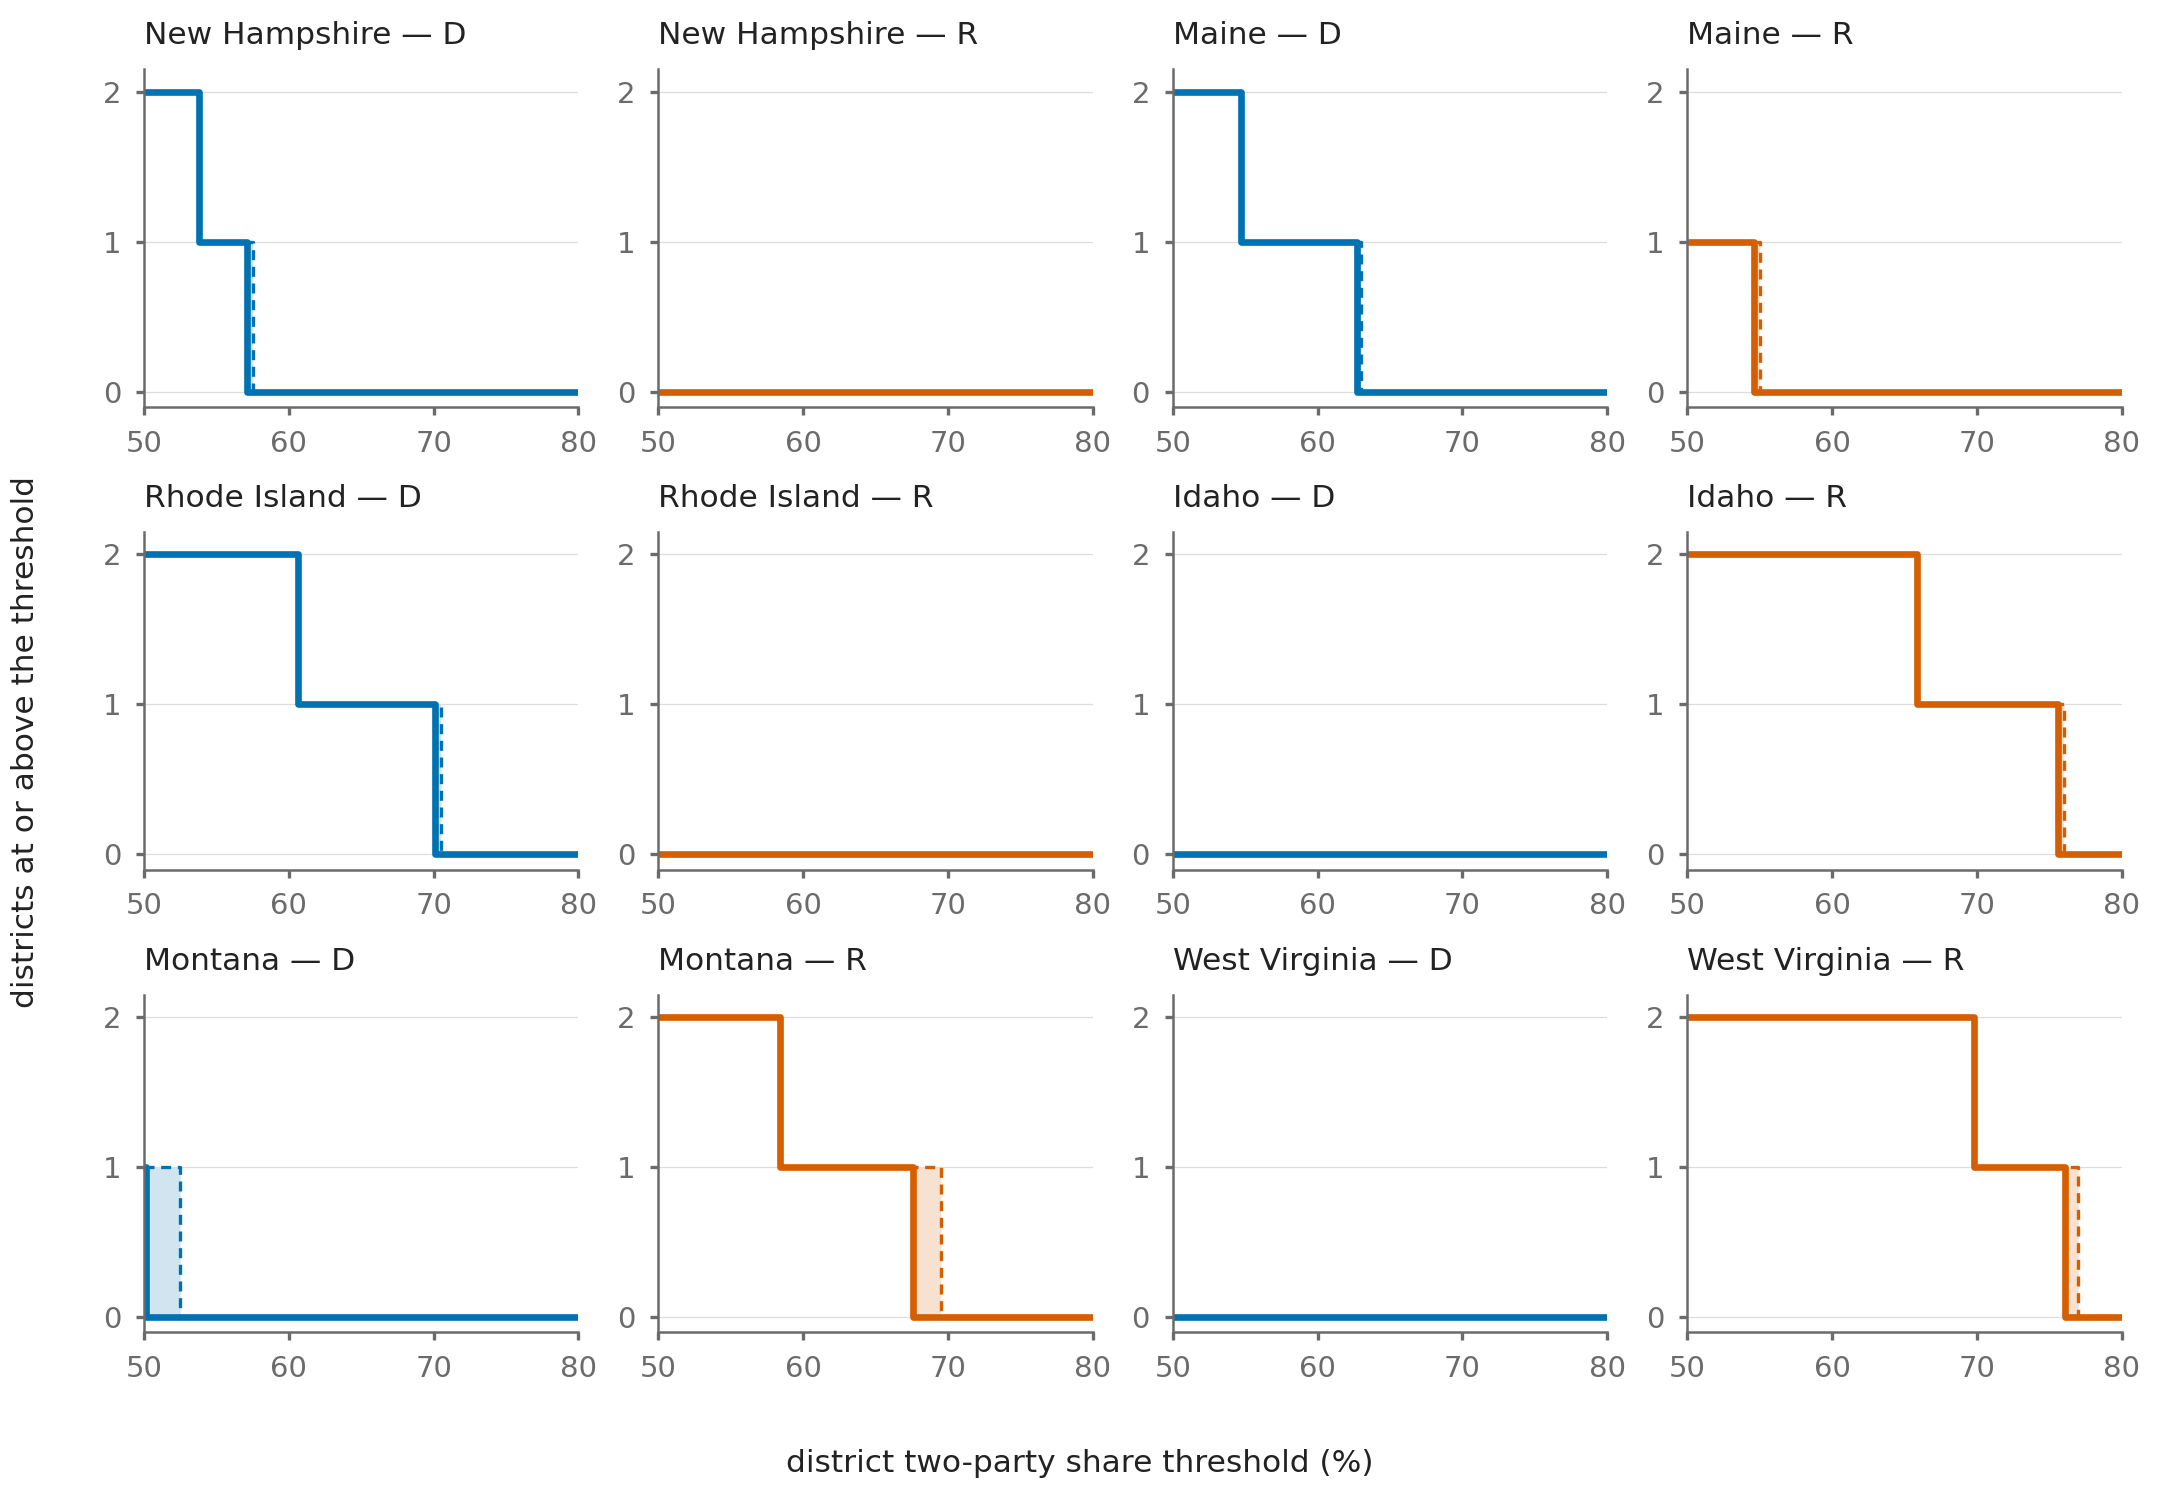
\includegraphics[width=\linewidth]{figs/frontier_k2.png}
\caption{Certified seat--safety frontiers $F(m)$ for the two-district states, both parties. Solid: certified lower staircase (independently verified plans); dashed: certified upper staircase (infeasibility proofs); shading: unresolved band. A party with no line above zero cannot make a district of that share in any plan of the regime.}\label{fig:frontier2}
\end{figure}

\paragraph{Exactness.}
At the three thresholds of Table~\ref{tab:capacity}, 79 of the 96 values of $F$ are pinned exactly: all 36 in the two-district states and 43 of the 60 in the states with three to five districts. Over a one-point grid of thresholds from 50\% to 80\%, 80\% of the 992 (state, party, threshold) values are exact. In terms of the spectrum (Table~\ref{tab:tightness}), 21 of the 24 brackets in the two-district states are tight to half a point of district share (median width 0.01 point once the geography-free bound is used as an additional upper bound) and the median bracket for $3\le k\le5$ is 2.2--2.6 points wide; the widest open brackets (9--14 points) are those of a party that is a minority in a state with three or more districts (Mississippi and Arkansas Democrats at $q=2$, Connecticut Democrats at $q=1$, Mississippi Republicans at $q=2$, Oklahoma Democrats).

\begin{table}[!tbp]
\centering\small
\caption{Width of the certified brackets $[r_q,u_q)$ for $\sigma^*(q)$, in points of district share, by number of districts $k$. Brackets proving that no $q$ districts can reach 50\% count as exact.}\label{tab:tightness}
\adjustbox{max width=\linewidth}{\begin{tabular}{crrrrrr}
\toprule
$k$ & brackets & exact ($\le0.5$ pt) & $\le1$ pt & $\le2$ pt & $\le3$ pt & median width (pts) \\
\midrule
2 & 24 & 21 & 22 & 23 & 24 & 0.01 \\
3 & 12 & 4 & 5 & 6 & 9 & 2.23 \\
4 & 48 & 10 & 12 & 19 & 27 & 2.62 \\
5 & 20 & 9 & 9 & 10 & 13 & 2.21 \\
\bottomrule
\end{tabular}
}
\end{table}

\paragraph{What the exact values say.}
(i) \emph{Certified zeros.} Republicans in New Hampshire and Rhode Island and Democrats in Idaho and West Virginia provably cannot make even one majority district (for Rhode Island, Idaho and West Virginia the geography-free bound already shows it; for New Hampshire Republicans it needs geography: the hull bound allows up to 54.6\%). (ii) \emph{Packing gains.} The best single district of a party can be far above the party's statewide share (Figure~\ref{fig:scatter}): for example Idaho Republicans (65.9\% statewide) can reach 75.5--76.0\%, Rhode Island Democrats (60.6\%) 70.0--70.5\%, and Maine Democrats (54.7\%) 62.7--63.0\% (Figure~\ref{fig:maps} shows witness plans for three of these states). (iii) \emph{The all-safe end is pinned by the statewide share.} Because the turnout-weighted mean of the district margins equals the statewide margin, $\sigma^*(k)$ cannot exceed it, and the resolved certified values sit within 0.2 point of it (Idaho Republicans $q=2$: 65.88\% against 65.9\%; Nebraska Republicans $q=3$: 59.71\% against 59.8\%; Connecticut Democrats $q=5$: 60.12\% against 60.2\%). (iv) \emph{A one-seat statement with geography.} Connecticut Republicans (39.8\% statewide) can make exactly one district with at least 50\%, and none with at least 55\%.

\begin{figure}[!tbp]
\centering
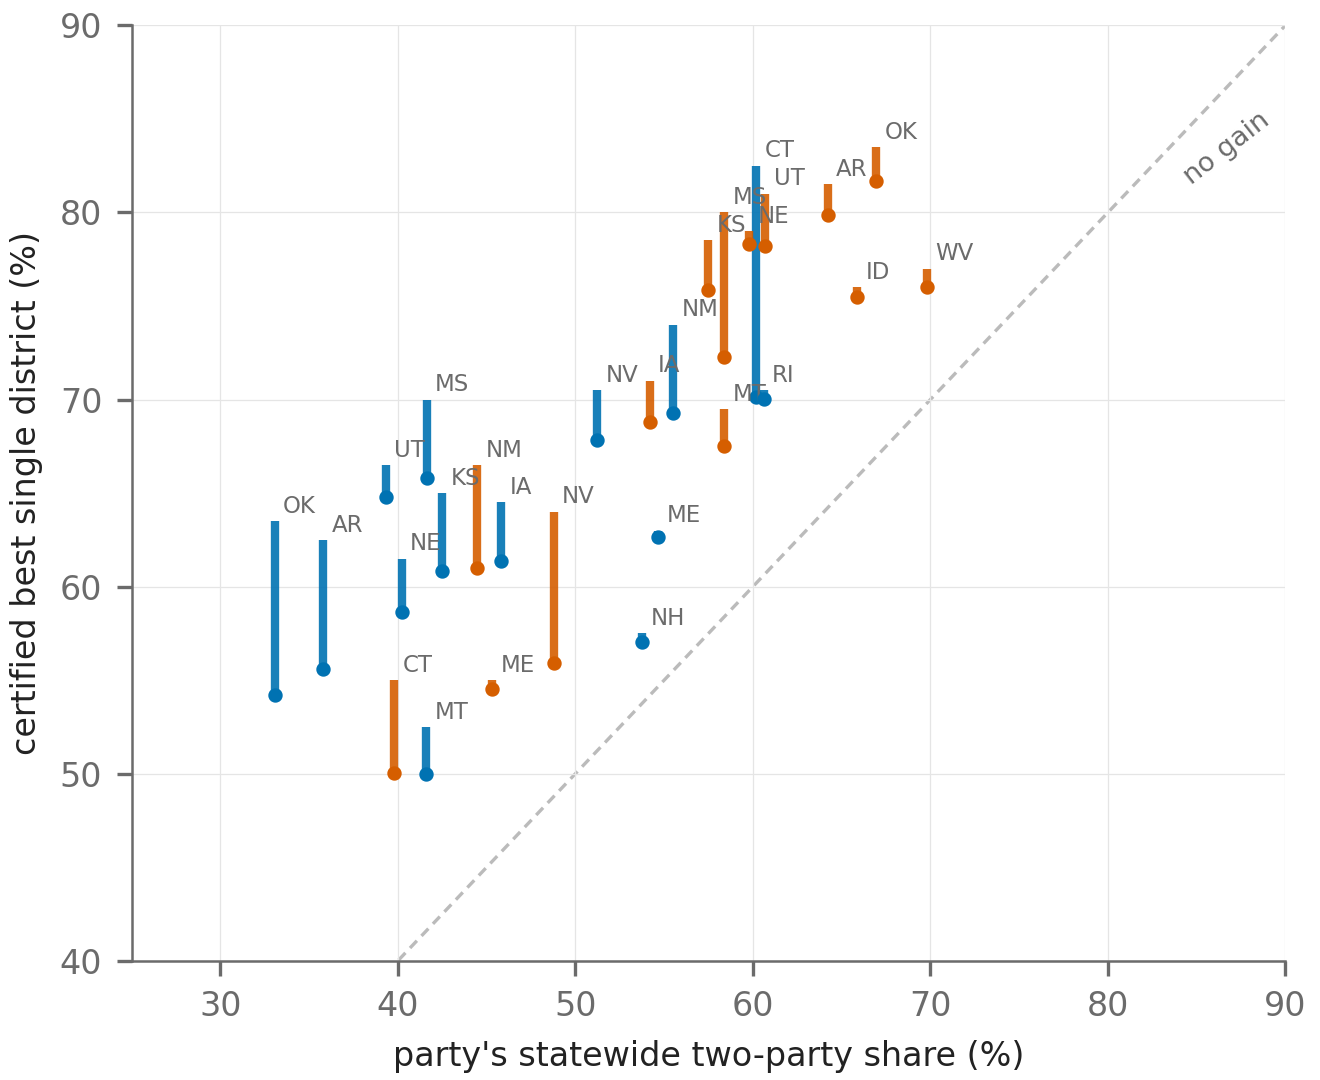
\includegraphics[width=\linewidth]{figs/scatter.png}
\caption{Certified bracket for the best single district ($q=1$) against the party's statewide two-party share. Points on the dashed diagonal would mean the boundaries give no gain.}\label{fig:scatter}
\end{figure}

\begin{figure}[!tbp]
\centering
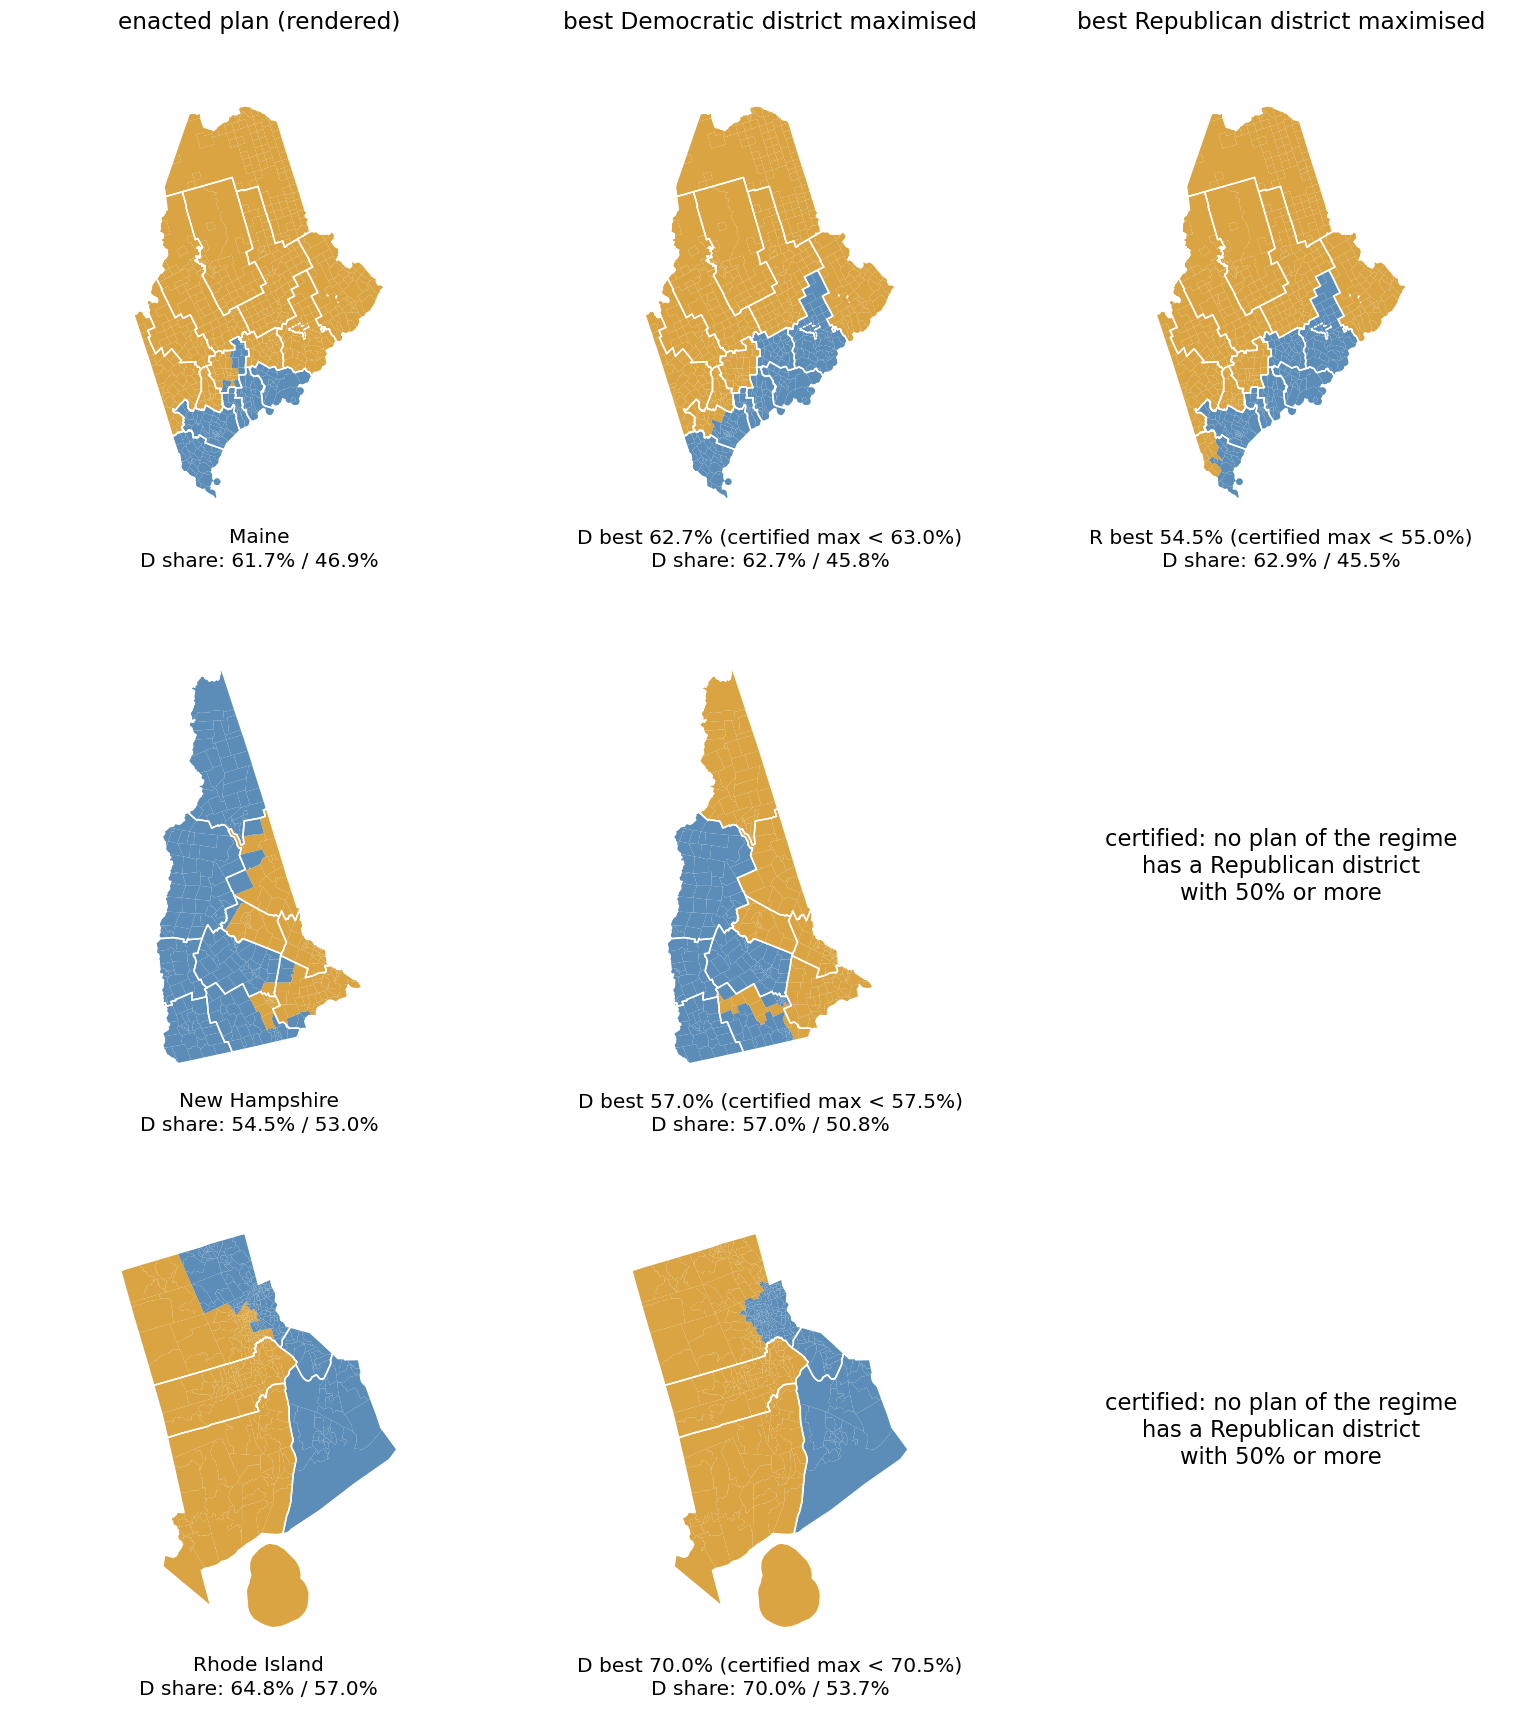
\includegraphics[width=0.9\linewidth,height=0.74\textheight,keepaspectratio]{figs/maps.png}
\caption{Witness plans of the certified brackets for Maine, New Hampshire and Rhode Island (two districts each). Left: the enacted plan rendered at precinct resolution. Middle and right: stored, independently verified plans that maximise the best Democratic (middle) and Republican (right) district; the certified upper end for the same quantity is in the panel title, so each plan is within the bracket width of the true optimum of the regime $\rho_s$. Where the proofs show that a party cannot reach 50\% in any district, no map is shown. Colours identify the district with the higher (blue) and lower (orange) Democratic share, not a party; white lines are county boundaries. These are witnesses that make the lower bounds checkable, not proposals.}\label{fig:maps}
\end{figure}

\begin{figure}[p]
\centering
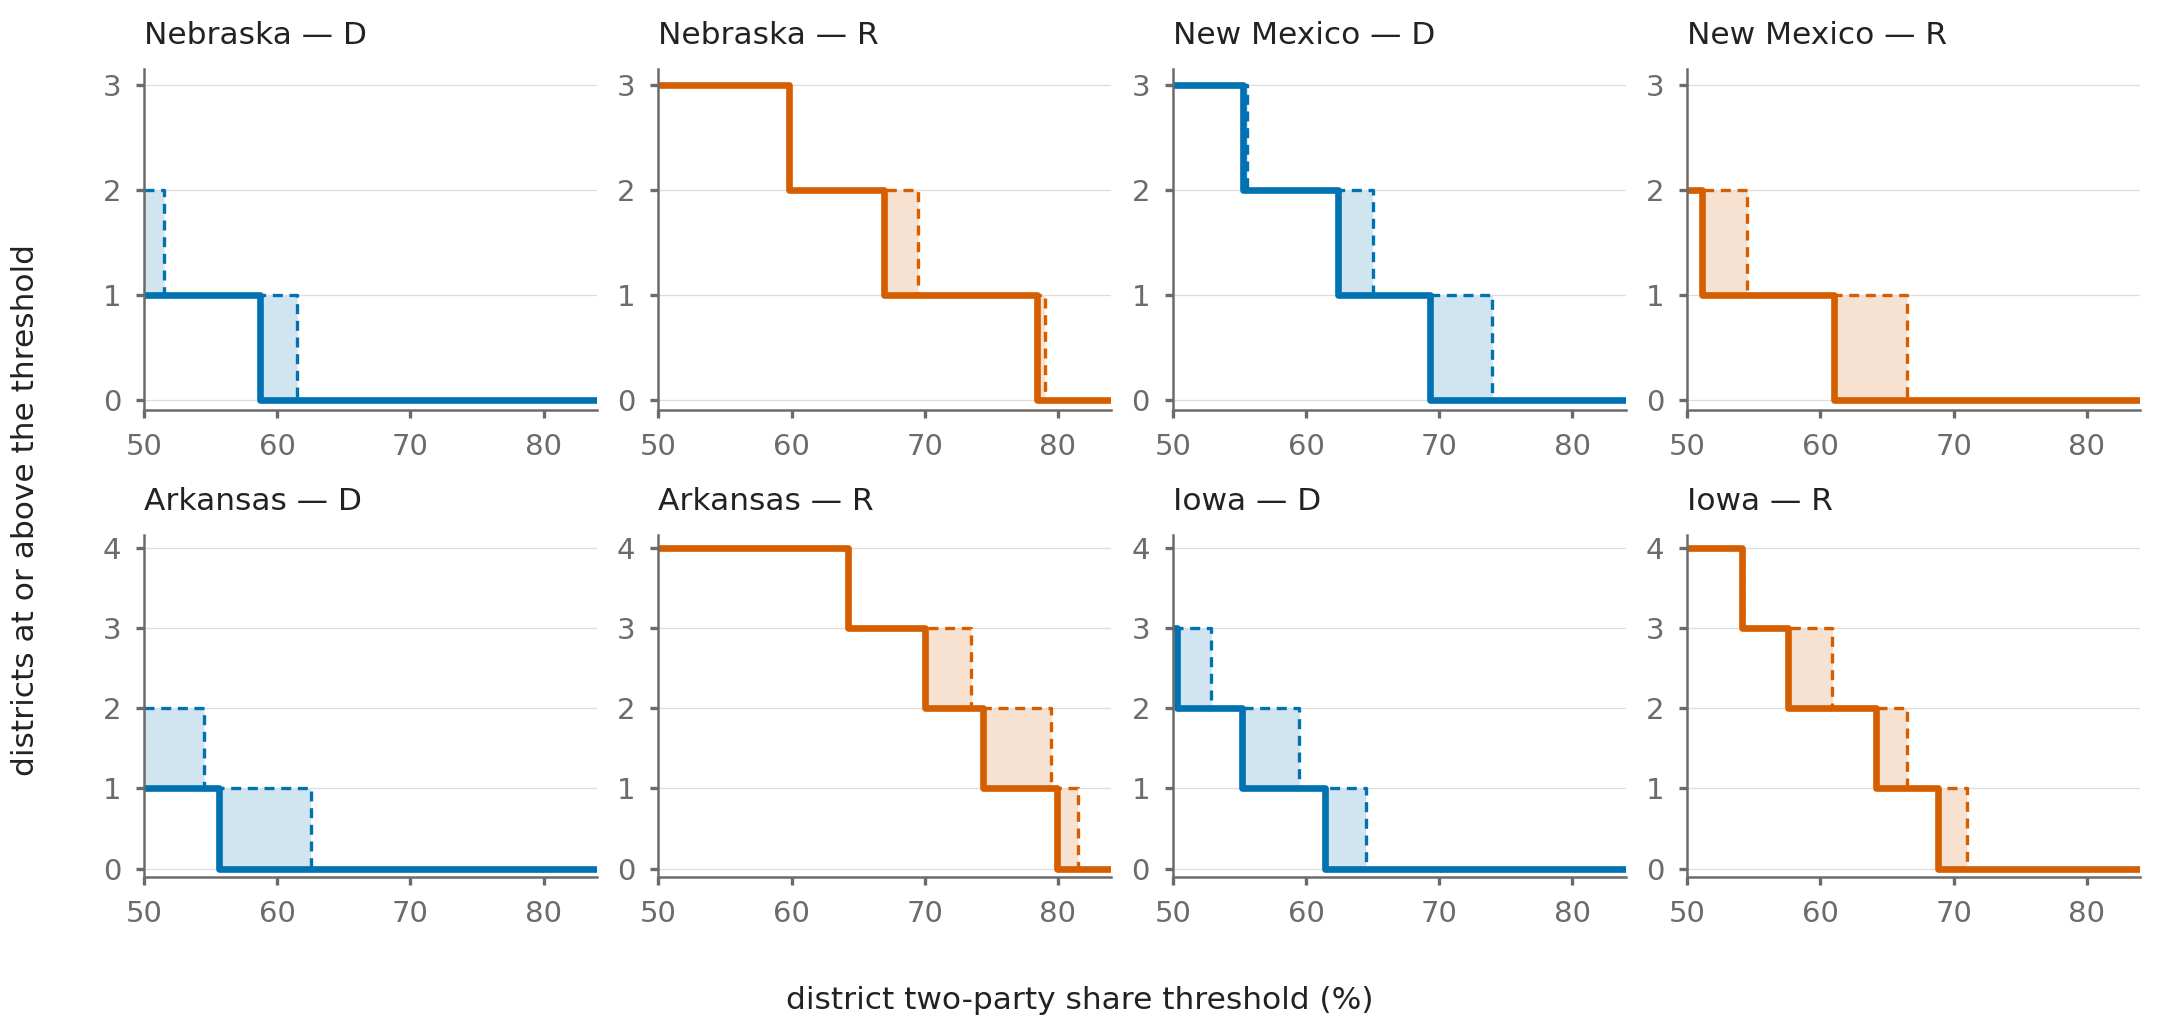
\includegraphics[width=\linewidth]{figs/frontier_k34a.png}\\[4pt]
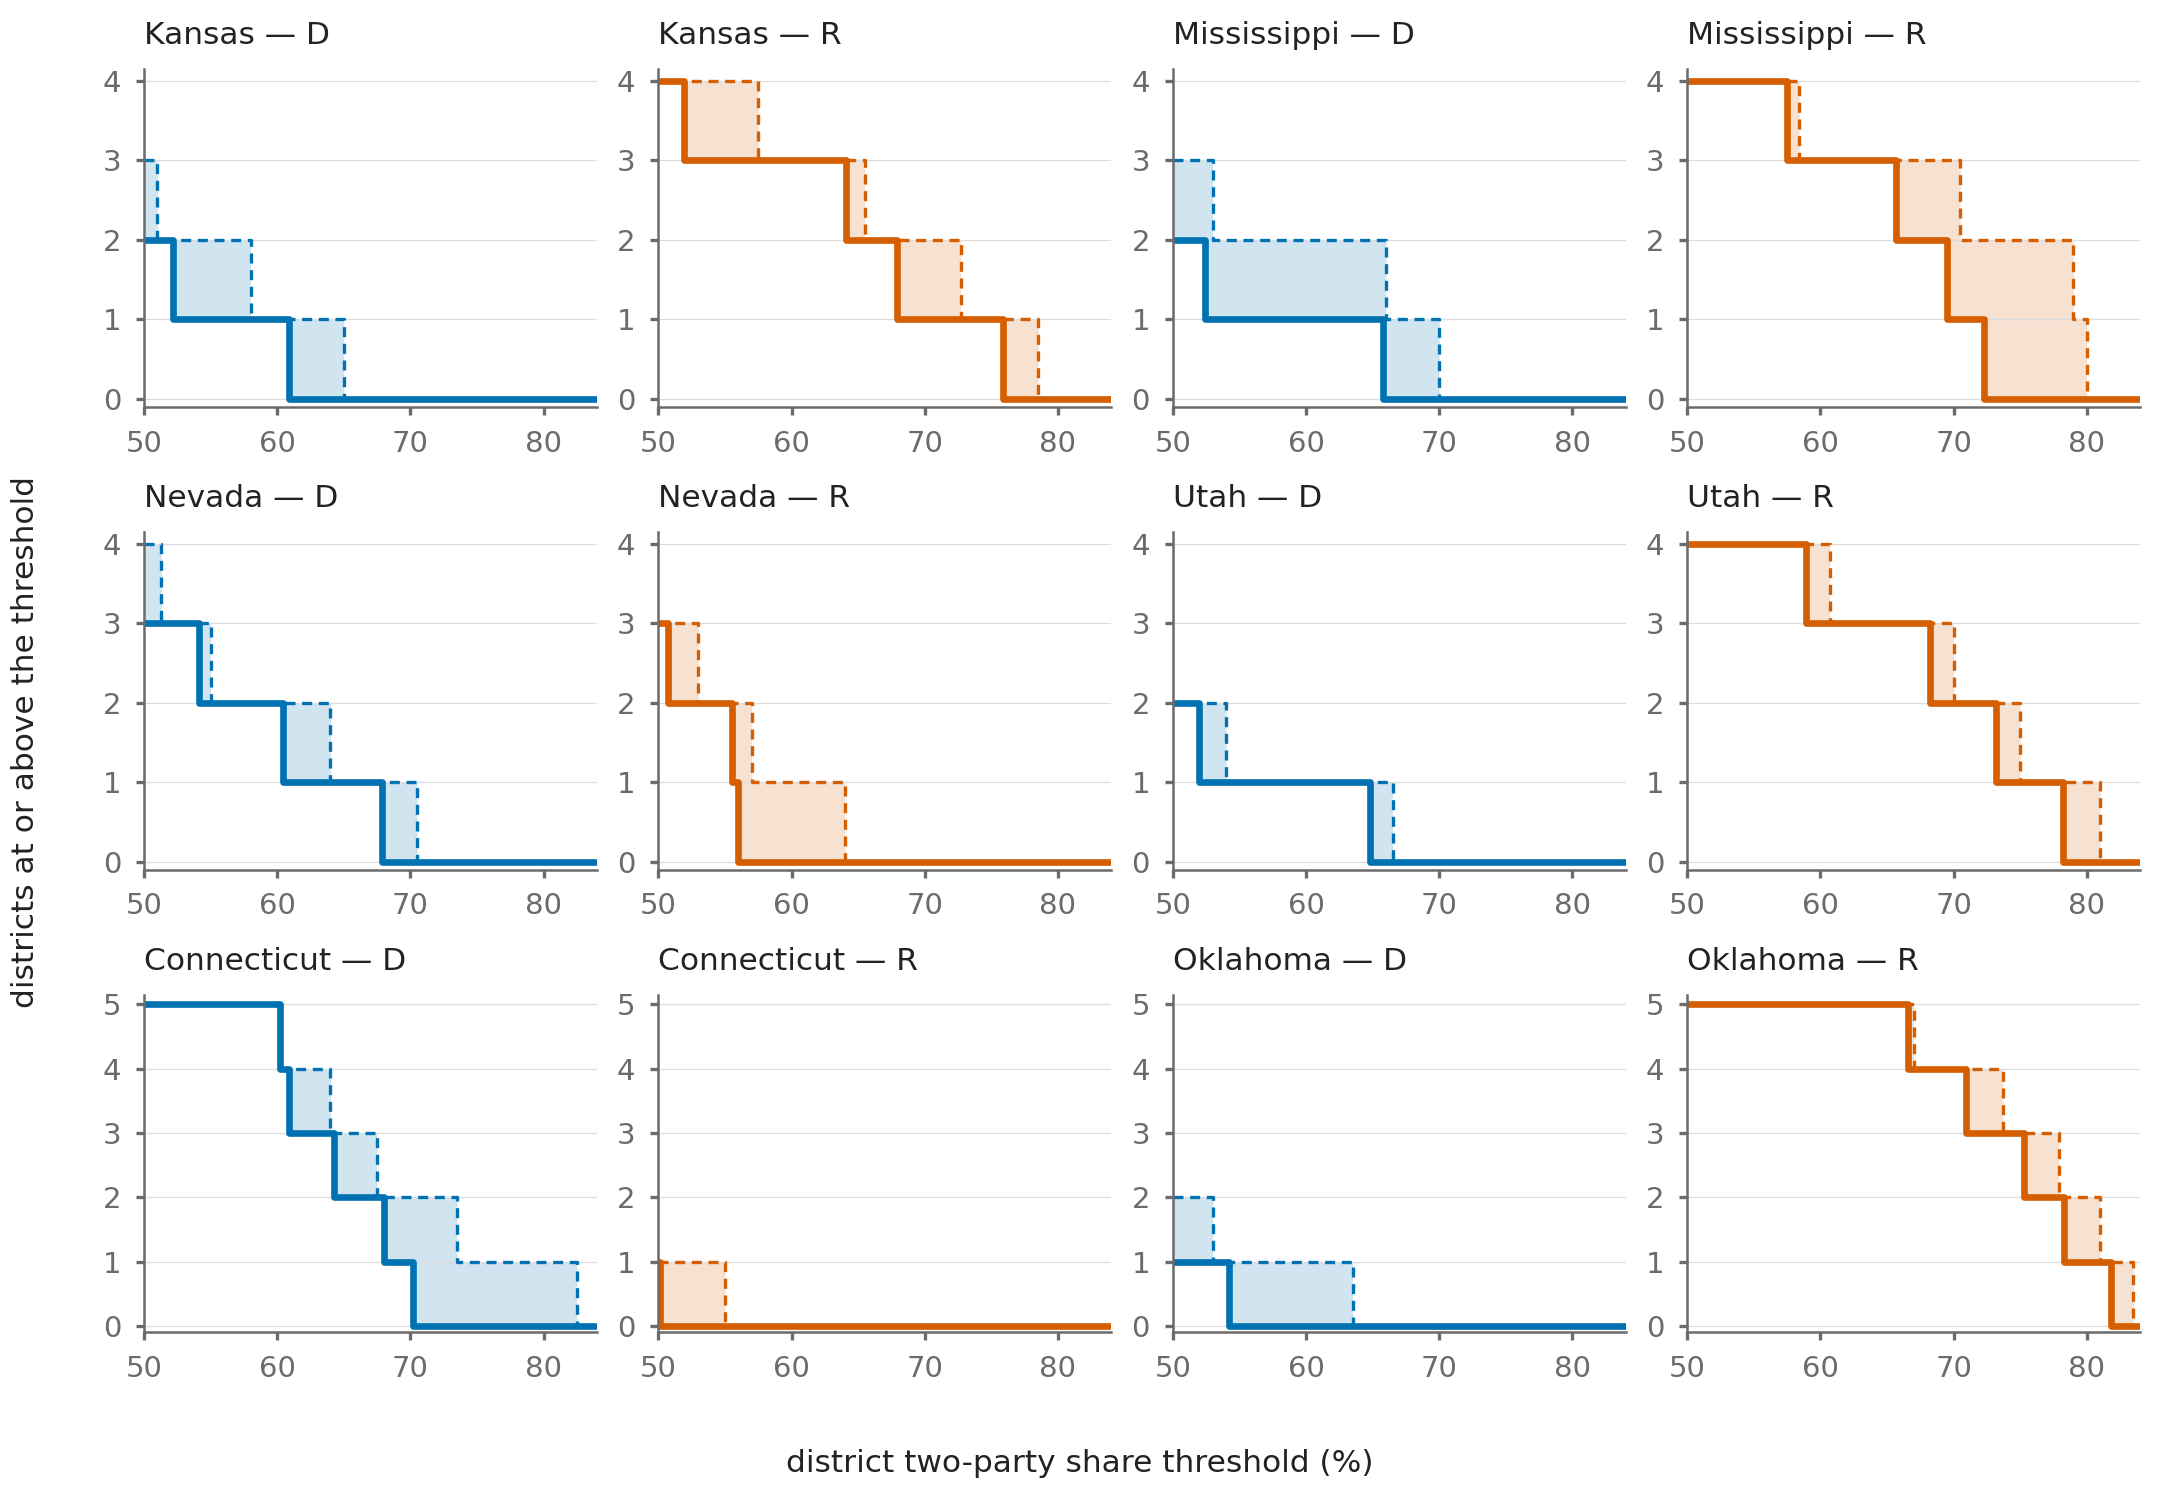
\includegraphics[width=\linewidth]{figs/frontier_k345b.png}
\caption{As Figure~\ref{fig:frontier2} for the states with three to five districts. Shaded bands mark brackets that remain open after the time limits of Section~\ref{sec:results}.}\label{fig:frontier3}
\end{figure}


\subsection{Seat ranges and the enacted plans in context}\label{sec:enacted}

The frontier at threshold $50\%$ has a direct seat interpretation. With two-party shares a district is Democratic-majority exactly when it is not Republican-majority, so under a regime $\rho$ the number of Democratic-majority districts of any plan lies between $k-F^{R}_\rho(0)$ and $F^{D}_\rho(0)$, and both ends are attained by some plan (Proposition~\ref{prop:mono}(4) gives the Republican side from the same code). Certified bounds on $F^D$ and $F^R$ therefore give a certified \emph{seat range} for each state; Table~\ref{tab:enacted} and Figure~\ref{fig:seatrange} report it next to the delegation of the enacted 118th-Congress plan and the seat count that would be proportional to the statewide vote. All counts use the two-party 2020 presidential vote in each district; they are descriptions of vote geography, not predictions of congressional results. (A district with an exactly tied two-party vote would count for both parties at threshold 50\%, so the range is exact up to such ties.)

\begin{table}[!tbp]
\centering\footnotesize
\caption{Seat range under $\rho_s$ at threshold 50\% and the enacted plans (2022 elections; each rendered at precinct resolution, Section~\ref{sec:data}). Columns give numbers of Democratic-majority districts: ``enacted'' for the enacted plan; ``verified'' the smallest and largest count attained by independently verified plans of $\rho_s$; ``limits'' what the infeasibility proofs leave possible. Splits are $\sum_K(d_K-1)$ of the rendered plan with the budget $s$ of $\rho_s$ in parentheses; ``in $\rho_s$'' says whether the rendered plan satisfies $\rho_s$ (population within $\pm1\%$, connected, at most $k-1$ splits).}\label{tab:enacted}
\adjustbox{max width=\linewidth}{\begin{tabular}{lrrcccrrc}
\toprule
State & $k$ & D share & enacted & verified & limits & splits ($s$) & max.\ dev. & in $\rho_s$ \\
\midrule
New Hampshire & 2 & 53.7\% & 2 & 2 & 2 & 5 (1) & 0.00\% & no \\
Maine & 2 & 54.7\% & 1 & 1--2 & 1--2 & 1 (1) & 0.00\% & yes \\
Rhode Island & 2 & 60.6\% & 2 & 2 & 2 & 1 (1) & 0.19\% & yes \\
Idaho & 2 & 34.1\% & 0 & 0 & 0 & 1 (1) & 0.02\% & yes \\
Montana & 2 & 41.6\% & 0 & 0--1 & 0--1 & 1 (1) & 0.07\% & no \\
West Virginia & 2 & 30.2\% & 0 & 0 & 0 & 0 (1) & 0.09\% & yes \\
Nebraska & 3 & 40.2\% & 1 & 0--1 & 0--2 & 2 (2) & 0.37\% & yes \\
New Mexico & 3 & 55.5\% & 3 & 1--3 & 1--3 & 10 (2) & 0.64\% & no \\
Arkansas & 4 & 35.8\% & 0 & 0--1 & 0--2 & 3 (3) & 0.05\% & yes \\
Iowa & 4 & 45.8\% & 0 & 0--3 & 0--3 & 0 (3) & 0.01\% & yes \\
Kansas & 4 & 42.5\% & 1 & 0--2 & 0--3 & 4 (3) & 0.05\% & no \\
Mississippi & 4 & 41.6\% & 1 & 0--2 & 0--3 & 4 (3) & 0.12\% & no \\
Nevada & 4 & 51.2\% & 3 & 1--3 & 1--4 & 3 (3) & 0.36\% & yes \\
Utah & 4 & 39.3\% & 0 & 0--2 & 0--2 & 7 (3) & 0.76\% & no \\
Connecticut & 5 & 60.2\% & 5 & 4--5 & 4--5 & 10 (4) & 0.77\% & no \\
Oklahoma & 5 & 33.1\% & 0 & 0--1 & 0--2 & 7 (4) & 0.21\% & no \\
\bottomrule
\end{tabular}
}
\end{table}

\begin{figure}[!tbp]
\centering
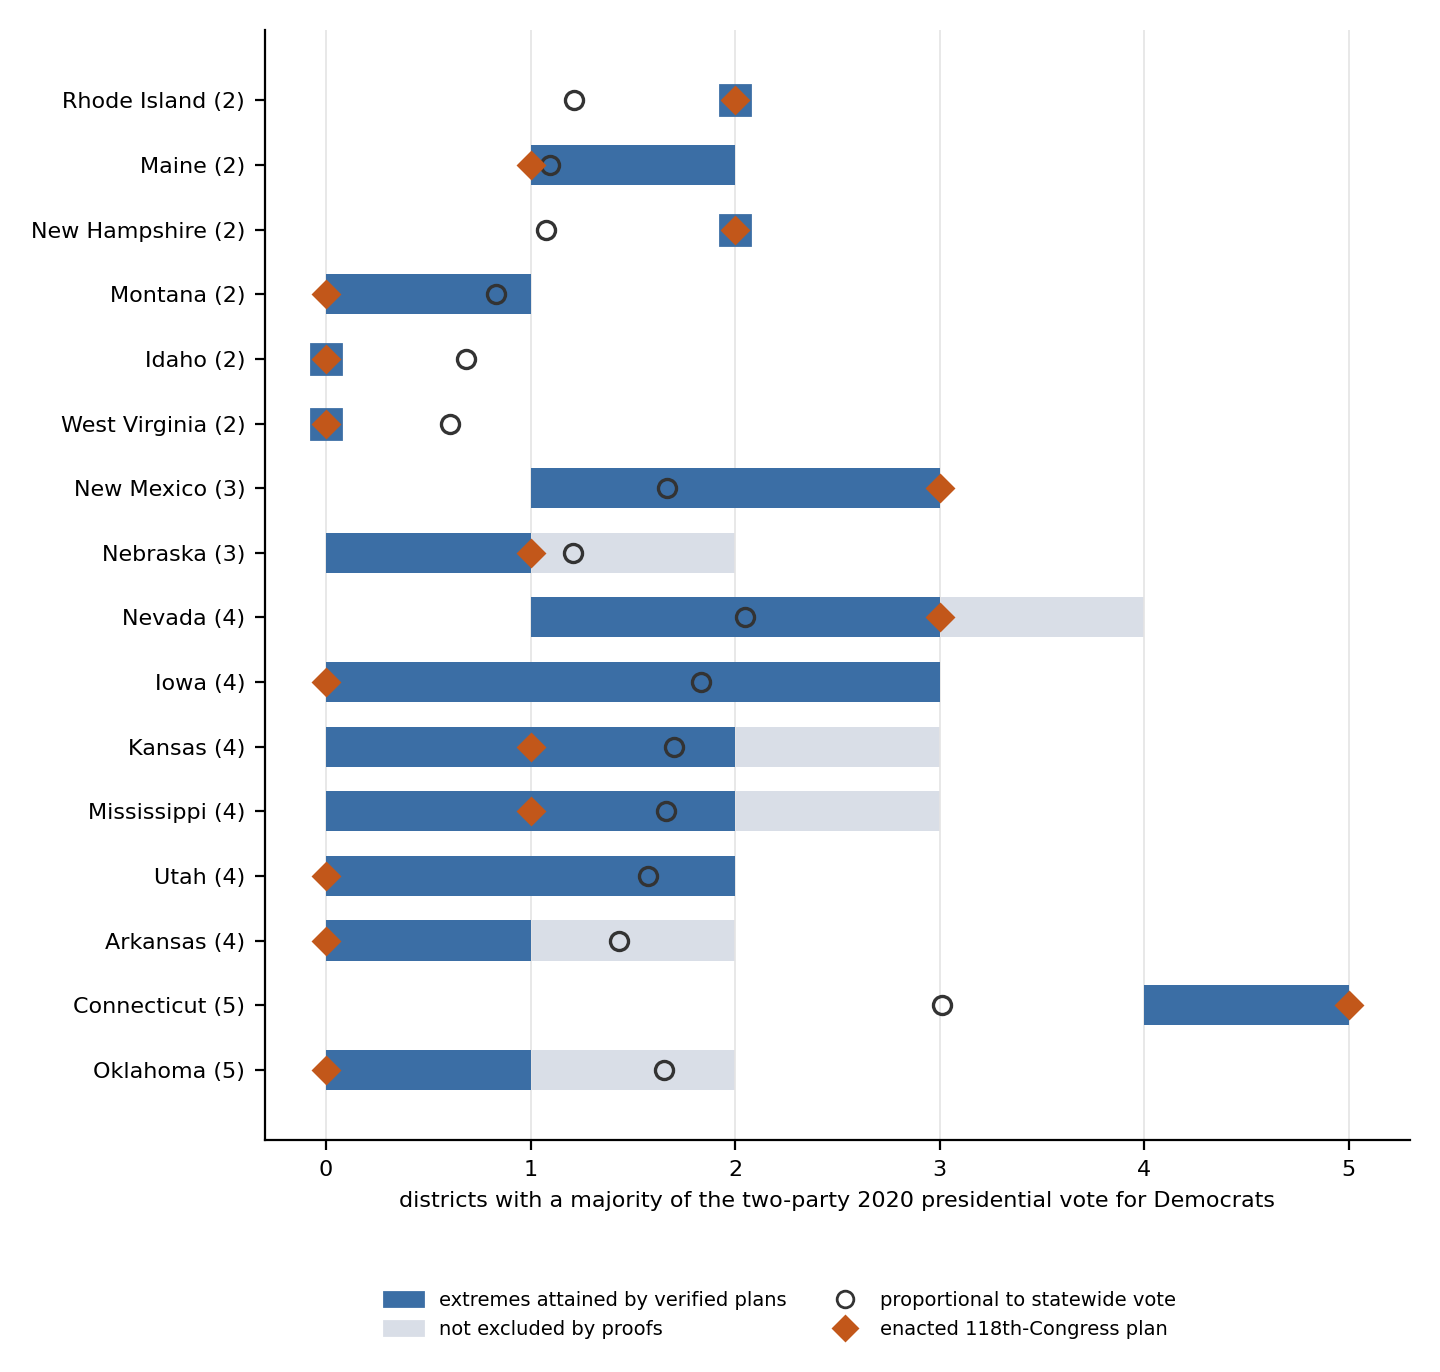
\includegraphics[width=0.86\linewidth,height=0.6\textheight,keepaspectratio]{figs/seatrange.png}
\caption{Certified range of the number of Democratic-majority districts under $\rho_s$ (threshold 50\% of the two-party 2020 presidential vote), the delegation of the enacted plan, and proportionality. Both extremes of the dark bar are attained by verified plans; light grey marks counts that the proofs do not exclude. Intermediate counts are not claimed to be attained.}\label{fig:seatrange}
\end{figure}

\paragraph{Where line drawing decides and where geography does.}
In four of the 16 states (New Hampshire and Rhode Island for Democrats, Idaho and West Virginia for Republicans) the delegation is the same for every plan of $\rho_s$: the two ends of the certified range coincide (Table~\ref{tab:enacted}). In the other twelve, verified plans attain a spread of one to three seats, and the proofs leave at most one further seat open in six of them; summed over the 52 seats of the 16 states, verified plans move the Democratic count between $11$ and $30$ and the proofs exclude anything below $11$ or above $36$ (the separability of Proposition~\ref{prop:sep} makes such sums valid for the union of states). Verified plans give Republicans a majority of the delegation in twelve of the 16 states and Democrats in seven; Iowa, Nevada and New Mexico are in both lists, and in New Hampshire, Rhode Island, Maine and Connecticut only Democrats can (in Maine Republicans can hold at most one of the two seats). Both parties are run through identical code, so which side has this capacity is a property of each state's vote geography and the regime. The Democratic delegations of the enacted plans total 19 of 52 seats (proportionality to the statewide votes would give 23.3), inside the verified range of 11 to 30.

\paragraph{The enacted plans in context.}
The rendered enacted plans are outside the regime in eight states, mainly because they split more counties than $k-1$ (Table~\ref{tab:enacted}; Montana's rendering has one detached precinct of 530 residents), and were drawn under criteria our model does not include, so their position relative to the range is a description and no evidence about intent. With that caveat, three observations are certified. First, in each of the 71 (state, party, $q$) combinations for which a verified plan has a $q$-th district above 50\%, the $q$-th best district of the enacted plan is below the certified lower end of $\sigma^*(q)$: by a median of 5.9 points of district share (5.4 points for the 28 single-best-district cases; smallest gap 0.2, largest 23.4; Figure~\ref{fig:scatter}, diamonds). No enacted plan exhausts what boundaries could do for either party at any rank, although a single plan cannot exhaust all ranks at once. Second, the delegation of the enacted plan lies at an end of the verified seat range in ten of the twelve states in which the range is not a single value, and in the interior in two (Kansas and Mississippi, each with one Democratic seat in a verified range of $0$--$2$); the end is the Republican end (fewest Democratic seats) in six of the ten and the Democratic end in four. Third, the enacted plans supply an independent test of the bounds: the eight of them that satisfy $\rho_s$ are ordinary plans of the regime, shaped by others (the test concerns the rendered plans, which are verified plans of $\rho_s$ whatever their fidelity to the enacted maps), and none of their 46 (party, $q$) margins reaches the proven upper end of the corresponding bracket, while none exceeds a lower end, so no plan in the public record improves our lower bounds in these states.


\subsection{Why the budget matters: connectivity coarsening alone does not help}\label{sec:negative}

The relaxation of Section~\ref{sec:relax} has two ingredients that can each tighten the geography-free bound: connectivity of the cell support in the quotient graph, and the subdivision budget. To separate them we ran, for every (state, party, $q$), (a) the geography-free hull bound (one cell, no connectivity: the sorting bound of \citealt{duchin2019}, extended to $k$-way allocations and the whole spectrum), (b) the aggregated relaxation with counties as cells and connectivity but \emph{no budget}, (c) the same after two uniform levels of refinement (roughly four to ten times as many cells), and compared them with the certified bracket under the budget $s=k-1$ (Figure~\ref{fig:ablation}, Table~\ref{tab:ablation} in the appendix; for $k\ge3$ the relaxations (a)--(c) are the pool relaxations with one aggregate for the unsafe districts, which are also valid).

\begin{figure}[!tbp]
\centering
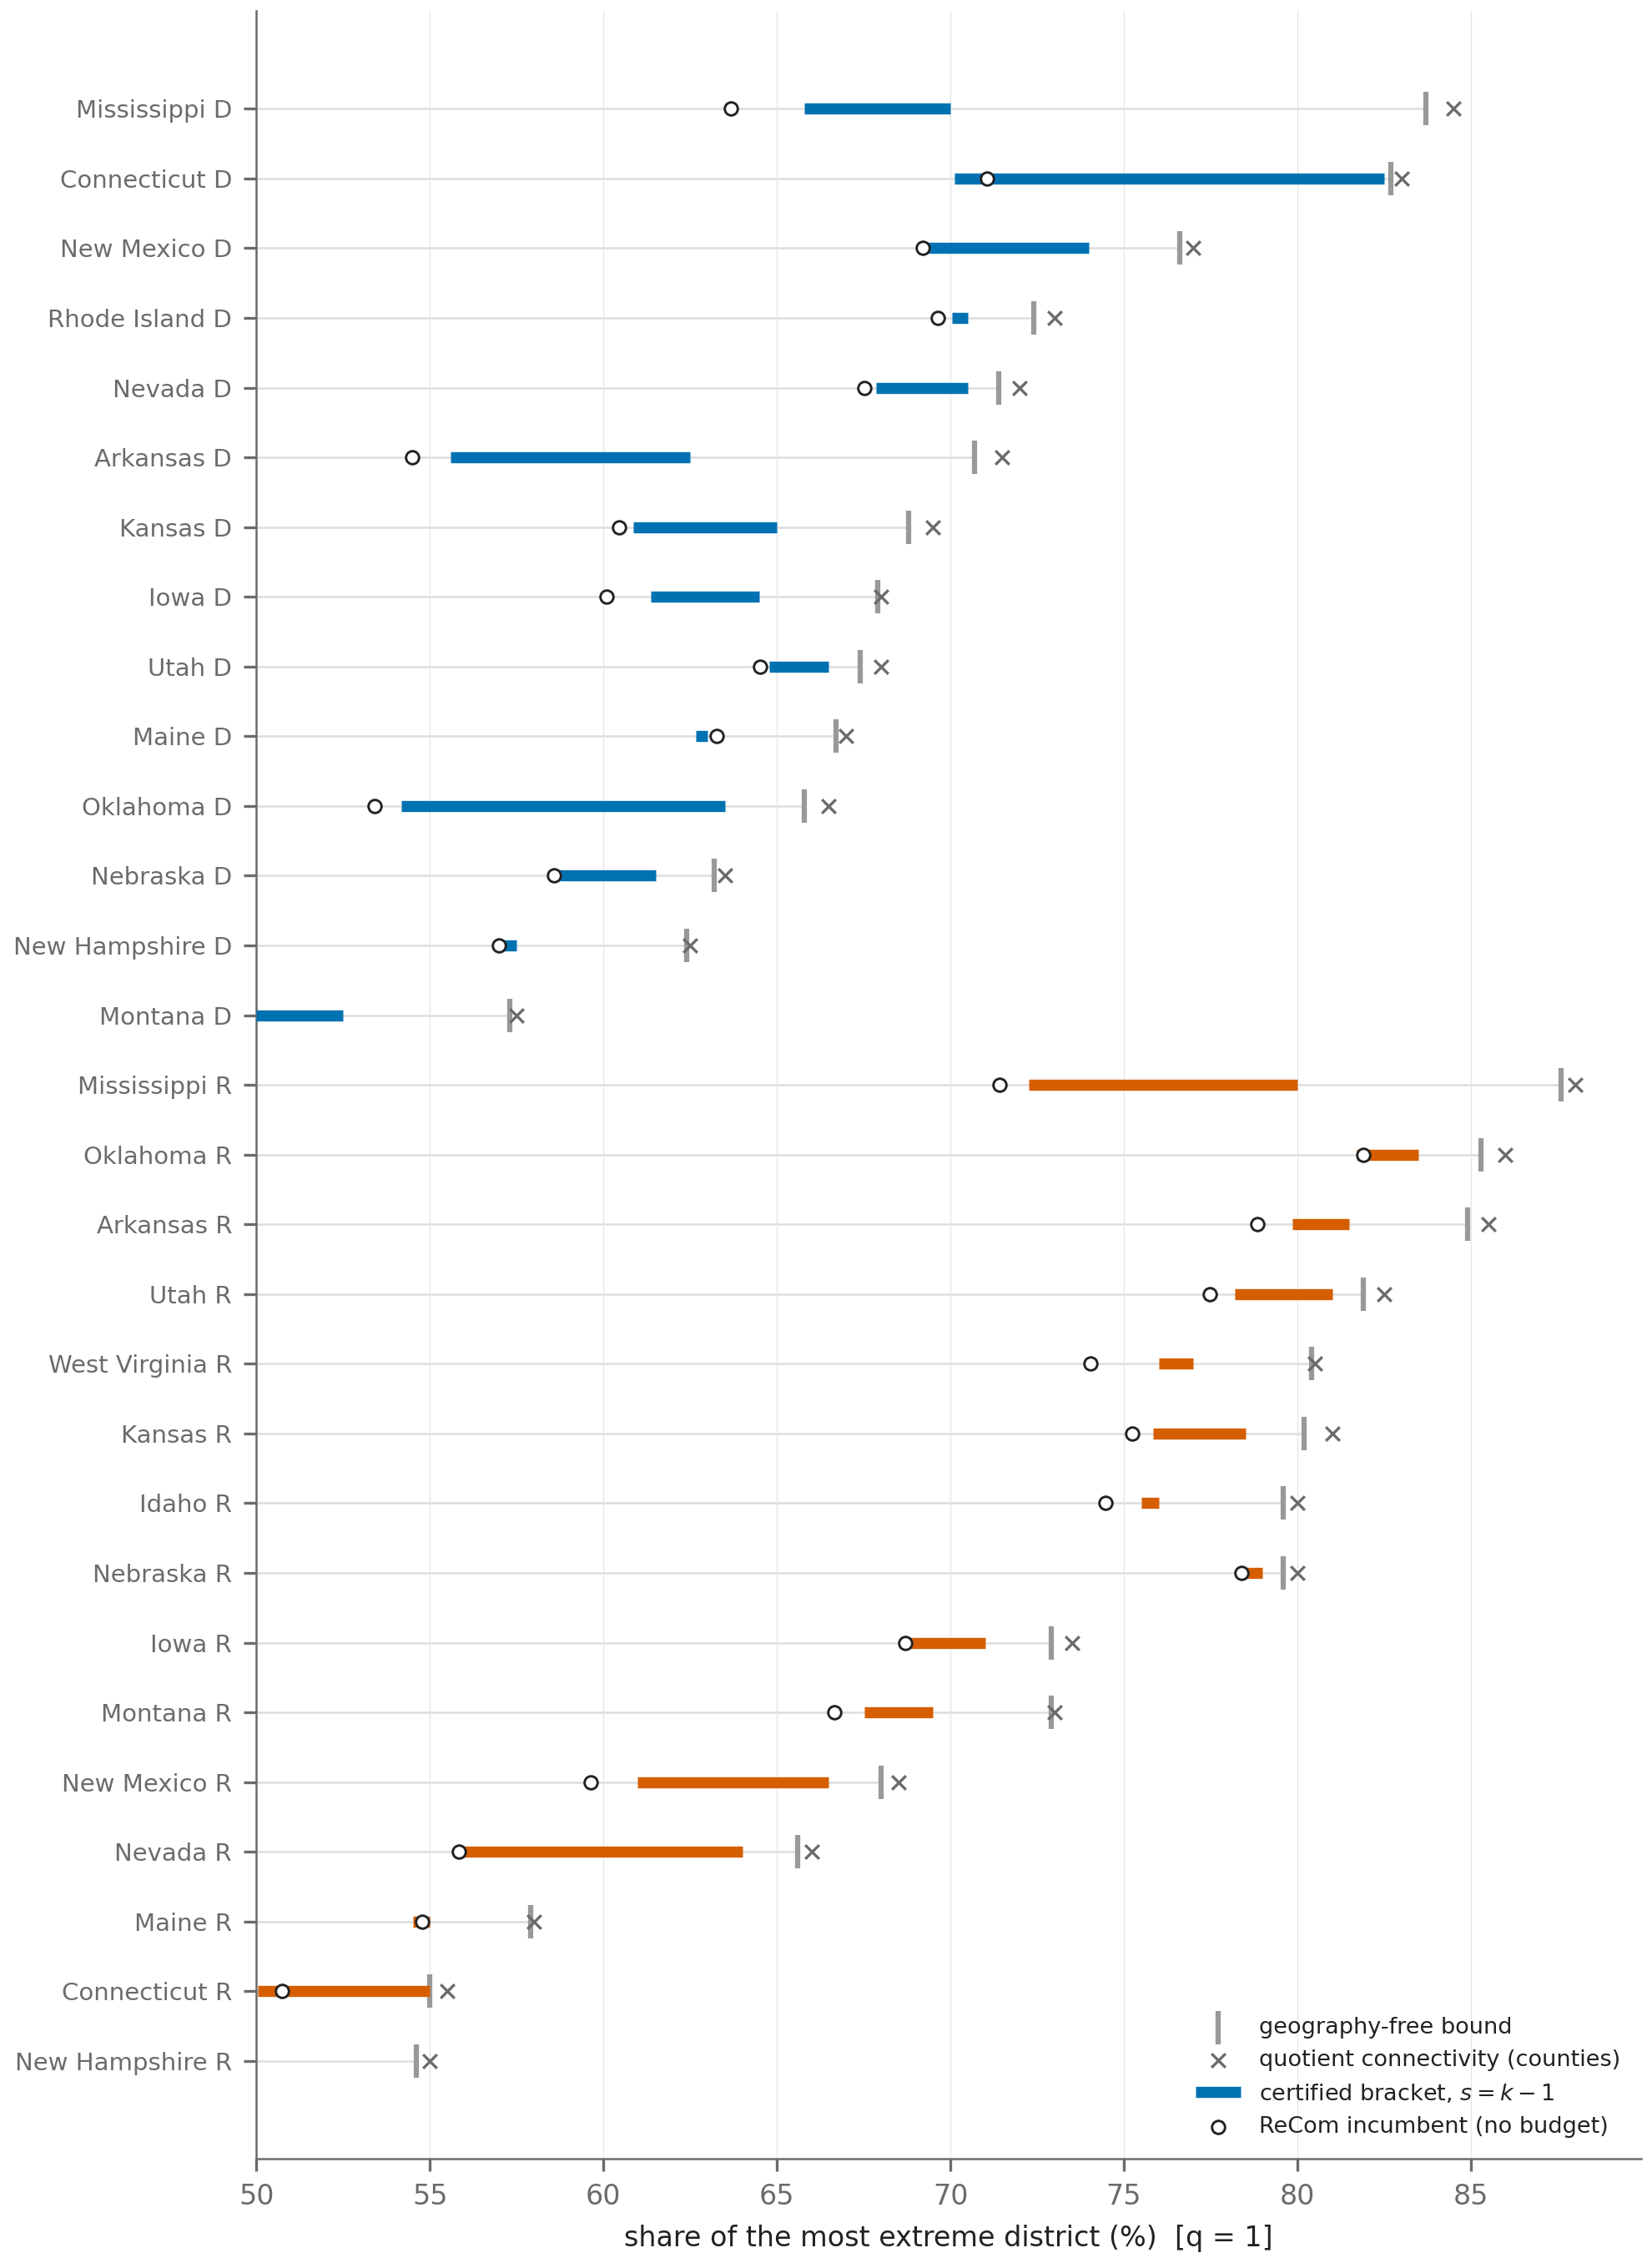
\includegraphics[width=\linewidth,height=0.68\textheight,keepaspectratio]{figs/ablation.png}
\caption{Upper bounds and incumbents for the share of the most extreme district ($q=1$), states with a nontrivial bound. Grey bar: geography-free hull bound; cross: quotient-connectivity relaxation with counties as cells and no budget (identical to within grid resolution after two further refinement levels); circle: 40-second unconstrained ReCom hill-climbing incumbent; thick bar: certified bracket under the budget of $k-1$ county splits.}\label{fig:ablation}
\end{figure}

\paragraph{Connectivity coarsening alone does nothing.}
Over the 79 nontrivial (state, party, $q$) triples the quotient relaxation without budget is never tighter than the geography-free bound (difference $+0.3$ point at the median, range 0.0 to $+0.8$, i.e. grid noise), and neither is it after two levels of refinement. This is the phenomenon of Proposition~\ref{prop:blind}: a district can touch every cell of a connected cell set while taking, in each cell, exactly its best atoms.

\paragraph{The budget does.}
The certified upper end under the budget is tighter than the geography-free bound by more than 0.05 point in 55 of the 78 triples with a finite upper end (median improvement 0.65 point; for $q=1$ the median is 2.75 points with a range from 0.2 to 13.7 points). Where it is not, the bracket is one of the open ones (Section~\ref{sec:main}) and the geography-free bound is used as the upper end (Table~\ref{tab:spectrum}). For the two-district states the improvement is decisive: New Hampshire Democrats 62.4\% $\to$ 57.0--57.5\%, Idaho Republicans 79.6\% $\to$ 75.5--76.0\%, West Virginia Republicans 80.4\% $\to$ 76.0--77.0\%.

\paragraph{Counting by pieces.}
Counting split \emph{counties} instead of pieces (a county cut among all districts costs one split) leaves a whole county as an unconstrained sub-problem. In development this was visible in Nebraska, where Douglas County holds 30\% of the state's population: under that convention the relaxed solutions of a query near the transition cut Douglas three ways for a single split, so that the exact problem contained a free three-way partition of 237 precincts, and CP-SAT alone could not even produce a feasible plan for $q=0$ within 300~s (a county-aware recombination heuristic finds one in milliseconds). We therefore adopted the piece-based count, which is also the convention of the exact county-split literature, and report only its results; we did not attempt a controlled comparison of the two conventions.


\subsection{Refinement versus monolithic exact solves}\label{sec:baseline}

Is the refinement loop needed, or would an exact solver on the atomic model do? We posed the 20 decision queries that produce the upper ends of the two-district brackets (for each state, party and rank the tightest margin at which the loop proved infeasibility; Table~\ref{tab:baseline}) to three exact methods under the same regime with a 300-second limit each: the CEGAR loop; CP-SAT on the atomic model of Section~\ref{sec:relax} (every precinct its own cell, exact parent-pointer connectivity and split row); and HiGHS on the independently written single-commodity-flow MILP of Section~\ref{sec:audit} on the atomic partition.

\begin{table}[!tbp]
\centering\footnotesize
\caption{Decision queries (``$q$ districts with share at least $m$?'', all answered ``no'' by the loop) posed to the CEGAR loop and to two monolithic exact solvers on the atomic model, 300 s limit, five CP-SAT workers (HiGHS: default threads). ``proof'' = proved infeasible; ``unknown'' = undecided at the limit. No solver returned a plan for a query that another proved infeasible.}\label{tab:baseline}
\adjustbox{max width=\linewidth}{\begin{tabular}{llcrrrr}
\toprule
State & Party & $q$ & margin $m$ & CEGAR & CP-SAT, atomic & HiGHS MILP, atomic \\
\midrule
Idaho & D & 1 & 50.0\% & proof ($<$1\,s) & proof (6\,s) & proof (2\,s) \\
Idaho & R & 1 & 76.0\% & proof (19\,s) & unknown ($>$300\,s) & unknown ($>$300\,s) \\
Idaho & R & 2 & 66.0\% & proof ($<$1\,s) & proof (1\,s) & proof (2\,s) \\
Maine & D & 1 & 63.0\% & proof ($<$1\,s) & proof (19\,s) & proof (41\,s) \\
Maine & D & 2 & 55.0\% & proof ($<$1\,s) & proof ($<$1\,s) & proof ($<$1\,s) \\
Maine & R & 1 & 55.0\% & proof ($<$1\,s) & proof (5\,s) & proof (2\,s) \\
Maine & R & 2 & 50.0\% & proof ($<$1\,s) & proof ($<$1\,s) & proof (1\,s) \\
Montana & D & 1 & 52.5\% & proof (91\,s) & unknown ($>$300\,s) & unknown ($>$300\,s) \\
Montana & D & 2 & 50.0\% & proof ($<$1\,s) & proof ($<$1\,s) & proof ($<$1\,s) \\
Montana & R & 1 & 69.5\% & proof (7\,s) & unknown ($>$300\,s) & unknown ($>$300\,s) \\
Montana & R & 2 & 58.5\% & proof ($<$1\,s) & proof (1\,s) & proof (1\,s) \\
New Hampshire & D & 1 & 57.5\% & proof ($<$1\,s) & unknown ($>$300\,s) & unknown ($>$300\,s) \\
New Hampshire & D & 2 & 54.0\% & proof ($<$1\,s) & proof ($<$1\,s) & proof ($<$1\,s) \\
New Hampshire & R & 1 & 50.0\% & proof ($<$1\,s) & unknown ($>$300\,s) & unknown ($>$300\,s) \\
Rhode Island & D & 1 & 70.5\% & proof (52\,s) & proof (19\,s) & unknown ($>$300\,s) \\
Rhode Island & D & 2 & 61.0\% & proof ($<$1\,s) & proof ($<$1\,s) & proof ($<$1\,s) \\
Rhode Island & R & 1 & 50.0\% & proof ($<$1\,s) & proof (1\,s) & proof ($<$1\,s) \\
West Virginia & D & 1 & 50.0\% & proof ($<$1\,s) & proof (11\,s) & proof (5\,s) \\
West Virginia & R & 1 & 77.0\% & proof (197\,s) & unknown ($>$300\,s) & unknown ($>$320\,s) \\
West Virginia & R & 2 & 70.0\% & proof ($<$1\,s) & proof (2\,s) & proof (7\,s) \\
\bottomrule
\end{tabular}
}
\end{table}

The loop decides all 20 (median 0.2 s; the slowest, West Virginia Republicans at 77\%, takes 197 s); atomic CP-SAT decides 14 and atomic HiGHS 13, and no two methods contradict each other, which is also a consistency check on the proofs (a plan returned where the loop proved infeasibility would refute the proof). The monolithic models are fast where the geography-free bound already nearly settles the query (every $q=2$ query and most zero-capacity queries: 0.3--41 s) and fail exactly on the seven best-district ($q=1$) queries near the transition margin, where the answer depends on how a county can be split. The largest contrast is New Hampshire: the county-level relaxation proves in about a tenth of a second (10 cells) that Democrats cannot reach 57.5\% and that Republicans cannot reach 50\% in any district, while neither monolithic solver decides either query in 300 s. The loop is not uniformly faster: atomic CP-SAT decides Rhode Island Democrats at 70.5\% in 19 s against 52 s for the loop. The comparison is between decision procedures under one time limit on one machine, not a statement about the best possible implementation of either.

\paragraph{Without the budget.}
The same test without a county-split budget ($s=\infty$) shows how much of the tractability comes from the budget. For three best-district queries---New Hampshire Democrats at 56\% and 58\%, Maine Democrats at 64\%---none of the three methods reaches a decision in 300 s: the loop has refined to 300--456 cells without a proof or a plan, and the atomic CP-SAT and HiGHS models return nothing, although a 40-second recombination run attains 57.0\% in New Hampshire, so the 56\% query is feasible. This agrees with the negative result: without the budget, certification of the interesting margins is out of reach for this method at precinct resolution, and it is the budget that turns the county level into an informative abstraction.


\subsection{Heuristic incumbents versus certified brackets}\label{sec:heur}

The lower ends of the brackets come from a county-aware recombination hill climber followed by exact large-neighbourhood search; to see what certification adds we compare them with the incumbent of a plain unconstrained ReCom short-burst run of 40~s per (state, party, $q$) with the same population tolerance (circles in Figure~\ref{fig:ablation}). This is a modest heuristic budget compared with the hours of computation behind published maps \citep{atlas2026}, so the comparison is illustrative rather than a ranking of methods.

\paragraph{Heuristics undershoot.}
The verified plans found under the budget (which is a restriction!) have a higher $q$-th margin than the unconstrained incumbent in 45 of 70 comparisons (median $+0.09$ point; range $-0.9$ to $+2.1$). In the largest cases the incumbent is one to two points below what is provably attainable: West Virginia Republicans 74.0\% against a certified 76.0--77.0\%, Idaho Republicans 74.5\% against 75.5--76.0\%.

\paragraph{A certified price of county integrity.}
In one case the unconstrained incumbent \emph{exceeds} the certified upper end: Maine Democrats reach 63.3\% in a verified unconstrained plan, whereas no plan of the budgeted regime reaches 63.0\%. Together the two facts are a certificate that the budget of one county split reduces the best-district capacity of Maine Democrats by at least 0.3 point at this tolerance. For every other state and party in our data the incumbent lies inside or below the bracket, so no separation is possible without a stronger unconstrained search or a certified upper bound for the unconstrained regime, which the negative result above suggests is out of reach at this resolution.


\subsection{Dependence on the subdivision budget}\label{sec:budget}

Table~\ref{tab:budget} reruns the two-district states New Hampshire, Maine and Rhode Island for budgets $s=1,\dots,4$ (the main regime is $s=1$). Brackets are closed under Proposition~\ref{prop:mono}(3): a plan that is feasible for $s$ is feasible for every larger budget, so the lower end at $s$ is the largest lower end over budgets $\le s$, and the upper end is the smallest over budgets $\ge s$ and the geography-free bound.

\begin{table}[t]
\centering\small
\caption{Best-district ($q=1$) and second-best ($q=2$) share, in percent of the two-party vote, as the county-split budget $s$ grows ($\pm1\%$, 2020 presidential vote); geography-free hull bound and unconstrained ReCom incumbent for comparison. ``$<$50'': no plan of the regime has $q$ districts at 50\% or more.}\label{tab:budget}
\begin{tabular}{llcccccrr}
\toprule
State & Party & $q$ & $s=1$ & $s=2$ & $s=3$ & $s=4$ & geo-free & ReCom (no budget) \\
\midrule
New Hampshire & D & 1 & 57.02--57.5 & 57.02--60.5 & 57.02--61.5 & 57.02--61.5 & 62.4 & 57.0 \\
New Hampshire & D & 2 & 53.75--53.8 & 53.75--53.8 & 53.75--53.8 & 53.75--53.8 & 53.8 & 53.7 \\
New Hampshire & R & 1 & $<$50 & 50.01--52.5 & 50.01--54.6 & 50.01--54.6 & 54.6 & -- \\
New Hampshire & R & 2 & $<$50 & $<$50 & $<$50 & $<$50 & $<$50 & -- \\
Maine & D & 1 & 62.67--63.0 & 63.87--64.0 & 64.07--64.5 & 64.51--65.0 & 66.7 & 63.3 \\
Maine & D & 2 & 54.62--54.7 & 54.62--54.7 & 54.62--54.7 & 54.62--54.7 & 54.7 & 54.6 \\
Maine & R & 1 & 54.52--55.0 & 55.54--56.0 & 55.82--56.0 & 56.02--56.5 & 57.9 & 54.8 \\
Maine & R & 2 & $<$50 & $<$50 & $<$50 & $<$50 & $<$50 & -- \\
Rhode Island & D & 1 & 70.04--70.5 & 70.04--71.5 & 70.37--72.4 & 70.37--72.4 & 72.4 & 69.6 \\
Rhode Island & D & 2 & 60.60--60.6 & 60.60--60.6 & 60.60--60.6 & 60.60--60.6 & 60.6 & 60.6 \\
Rhode Island & R & 1 & $<$50 & $<$50 & $<$50 & $<$50 & $<$50 & -- \\
Rhode Island & R & 2 & $<$50 & $<$50 & $<$50 & $<$50 & $<$50 & -- \\
Idaho & D & 1 & $<$50 & $<$50 & $<$50 & $<$50 & $<$50 & -- \\
Idaho & D & 2 & $<$50 & $<$50 & $<$50 & $<$50 & $<$50 & -- \\
Idaho & R & 1 & 75.50--76.0 & 75.88--77.0 & 75.88--78.0 & 75.88--78.0 & 79.6 & 74.5 \\
Idaho & R & 2 & 65.88--65.9 & 65.88--65.9 & 65.88--65.9 & 65.88--65.9 & 65.9 & 65.9 \\
Montana & D & 1 & 50.00--52.5 & 50.00--57.3 & 50.00--57.3 & 50.00--57.3 & 57.3 & -- \\
Montana & D & 2 & $<$50 & $<$50 & $<$50 & $<$50 & $<$50 & -- \\
Montana & R & 1 & 67.53--69.5 & 67.53--71.0 & 68.38--71.0 & 68.38--72.9 & 72.9 & 66.6 \\
Montana & R & 2 & 58.40--58.4 & 58.40--58.4 & 58.40--58.4 & 58.40--58.4 & 58.4 & 58.4 \\
West Virginia & D & 1 & $<$50 & $<$50 & $<$50 & $<$50 & $<$50 & -- \\
West Virginia & D & 2 & $<$50 & $<$50 & $<$50 & $<$50 & $<$50 & -- \\
West Virginia & R & 1 & 76.00--77.0 & 76.00--77.5 & 76.00--79.0 & 76.00--79.5 & 80.4 & 74.0 \\
West Virginia & R & 2 & 69.78--69.8 & 69.78--69.8 & 69.79--69.8 & 69.79--69.8 & 69.8 & 69.8 \\
\bottomrule
\end{tabular}

\end{table}

\paragraph{Capacity grows with every split, provably.}
For Maine the certified best-district share of Democrats is 62.67--63.0\% at $s=1$, 63.87--64.0\% at $s=2$, 64.07--64.5\% at $s=3$ and 64.51--65.0\% at $s=4$ (Republicans: 54.5--55.0, 55.5--56.0, 55.8--56.0, 56.0--56.5\%). Wherever the upper end of one budget lies below the lower end of the next (Maine $s=1\to2$ for both parties, Democrats $s=2\to3$ and $3\to4$, Republicans $3\to4$), the extra split is \emph{certified} to increase capacity, by at least 0.8 point for the first split of Maine Democrats. The geography-free bound (66.7\% and 57.9\%) is far above even $s=4$: contiguity and the remaining budget, not the vote totals alone, bind in these states.

\paragraph{A seat-level effect.}
New Hampshire Republicans cannot make a single 50\% district with one split (certified), but can with two: a verified plan has a 50.01\% district. The frontier therefore moves by a whole seat at the first extra split.

\paragraph{The all-safe end does not depend on the budget.}
$\sigma^*(2)$ is pinned to the statewide share for every budget tried (New Hampshire 53.75--53.8\%, Maine 54.62--54.7\%, Rhode Island 60.60\%), as it must be when the largest possible value equals the statewide margin (Section~\ref{sec:main}).

\paragraph{Tractability.}
Exactness is lost when the budget grows in New Hampshire (upper end for Democrats 57.5\% at $s=1$, 60.5\% at $s=2$, 61.5\% at $s\ge3$) and Rhode Island, but not in Maine, where every bracket is at most half a point wide for $s\le4$. This is the tractability frontier of the method: it depends on the budget and on the structure of the counties (Maine has 16), and it is where a relaxed solution has room to cheat inside a split county.


\subsection{Robustness: tolerance, scenarios and resolution}\label{sec:robust}

\paragraph{Tolerance and scenario set.}
Table~\ref{tab:robust} varies the population tolerance $\varepsilon\in\{0.5\%,1\%,2\%\}$ (single scenario, $s=k-1$) and replaces the single 2020 presidential race by the minimum share over up to three statewide contests (presidential, and where available Senate and governor), for the six two-district states. Brackets are closed under Proposition~\ref{prop:mono} (a larger tolerance can only raise both ends; a larger scenario set can only lower them).

\begin{table}[!tbp]
\centering\small
\caption{Best-district ($q=1$) and second-best ($q=2$) share (\%) for tolerances 0.5\%, 1\% and 2\%, and for the robust scenario set at 1\% (number of contests in the last column). $s=k-1=1$.}\label{tab:robust}
\adjustbox{max width=\linewidth}{\begin{tabular}{llcccccc}
\toprule
State & Party & $q$ & $\varepsilon{=}0.5\%$ & $\varepsilon{=}1\%$ & $\varepsilon{=}2\%$ & robust $\Omega$, 1\% & contests \\
\midrule
New Hampshire & D & 1 & 57.01--57.5 & 57.02--57.5 & 57.14--57.5 & $<$50 & 3 \\
New Hampshire & D & 2 & 53.75--54.0 & 53.75--54.0 & 53.75--54.0 & $<$50 & 3 \\
New Hampshire & R & 1 & $<$50 & $<$50 & $<$50 & $<$50 & 3 \\
New Hampshire & R & 2 & $<$50 & $<$50 & $<$50 & $<$50 & 3 \\
Maine & D & 1 & 62.74--63.0 & 62.74--63.0 & 63.12--63.5 & 53.19--53.5 & 2 \\
Maine & D & 2 & 54.62--55.0 & 54.62--55.0 & 54.65--55.0 & $<$50 & 2 \\
Maine & R & 1 & 54.51--55.0 & 54.52--55.0 & 54.58--55.0 & 54.53--55.0 & 2 \\
Maine & R & 2 & $<$50 & $<$50 & $<$50 & $<$50 & 2 \\
Rhode Island & D & 1 & 70.12--70.5 & 70.12--70.5 & 70.52--71.0 & 70.31--70.5 & 2 \\
Rhode Island & D & 2 & 60.60--61.0 & 60.60--61.0 & 60.60--61.0 & 60.60--61.0 & 2 \\
Rhode Island & R & 1 & $<$50 & $<$50 & $<$50 & $<$50 & 2 \\
Rhode Island & R & 2 & $<$50 & $<$50 & $<$50 & $<$50 & 2 \\
Idaho & D & 1 & $<$50 & $<$50 & $<$50 & $<$50 & 2 \\
Idaho & D & 2 & $<$50 & $<$50 & $<$50 & $<$50 & 2 \\
Idaho & R & 1 & 75.52--76.0 & 75.52--76.0 & 75.62--76.5 & 74.53--75.5 & 2 \\
Idaho & R & 2 & 65.87--66.0 & 65.88--66.0 & 65.88--66.0 & 65.32--65.5 & 2 \\
West Virginia & D & 1 & $<$50 & $<$50 & $<$50 & $<$50 & 3 \\
West Virginia & D & 2 & $<$50 & $<$50 & $<$50 & $<$50 & 3 \\
West Virginia & R & 1 & 74.57--77.0 & 76.00--77.0 & 76.00--77.5 & 73.13--75.5 & 3 \\
West Virginia & R & 2 & 69.79--70.0 & 69.79--70.0 & 69.79--70.0 & 67.75--68.0 & 3 \\
\bottomrule
\end{tabular}
}
\end{table}

The tolerance matters little: doubling it from 1\% to 2\% shifts the certified bracket of the best district up by 0.4--0.5 point in Maine (Democrats) and Rhode Island (Democrats), where the two brackets are disjoint and the increase is therefore certified, by up to 0.1 point in New Hampshire, and by less than the bracket width elsewhere. Requiring the margin to hold in \emph{all} available contests matters a great deal for parties that did worse in the other races: New Hampshire Democrats, whose 57\% district relies on the presidential vote alone, can no longer make any district above 50\% in all of presidential, Senate and gubernatorial results (the 2020 governor's race was a Republican landslide); Maine Democrats fall from 62.7--63.0\% to 53.2--53.5\%; West Virginia Republicans from 76.0--77.0\% to 73.1--75.5\%; Montana Republicans from 67.5--69.5\% to 63.6--67.0\%. Rhode Island Democrats and Maine Republicans are unaffected. The seat--safety spectrum therefore doubles as a durability measure: the share cushion a district retains across elections is exactly its robust margin.

\begin{figure}[!tbp]
\centering
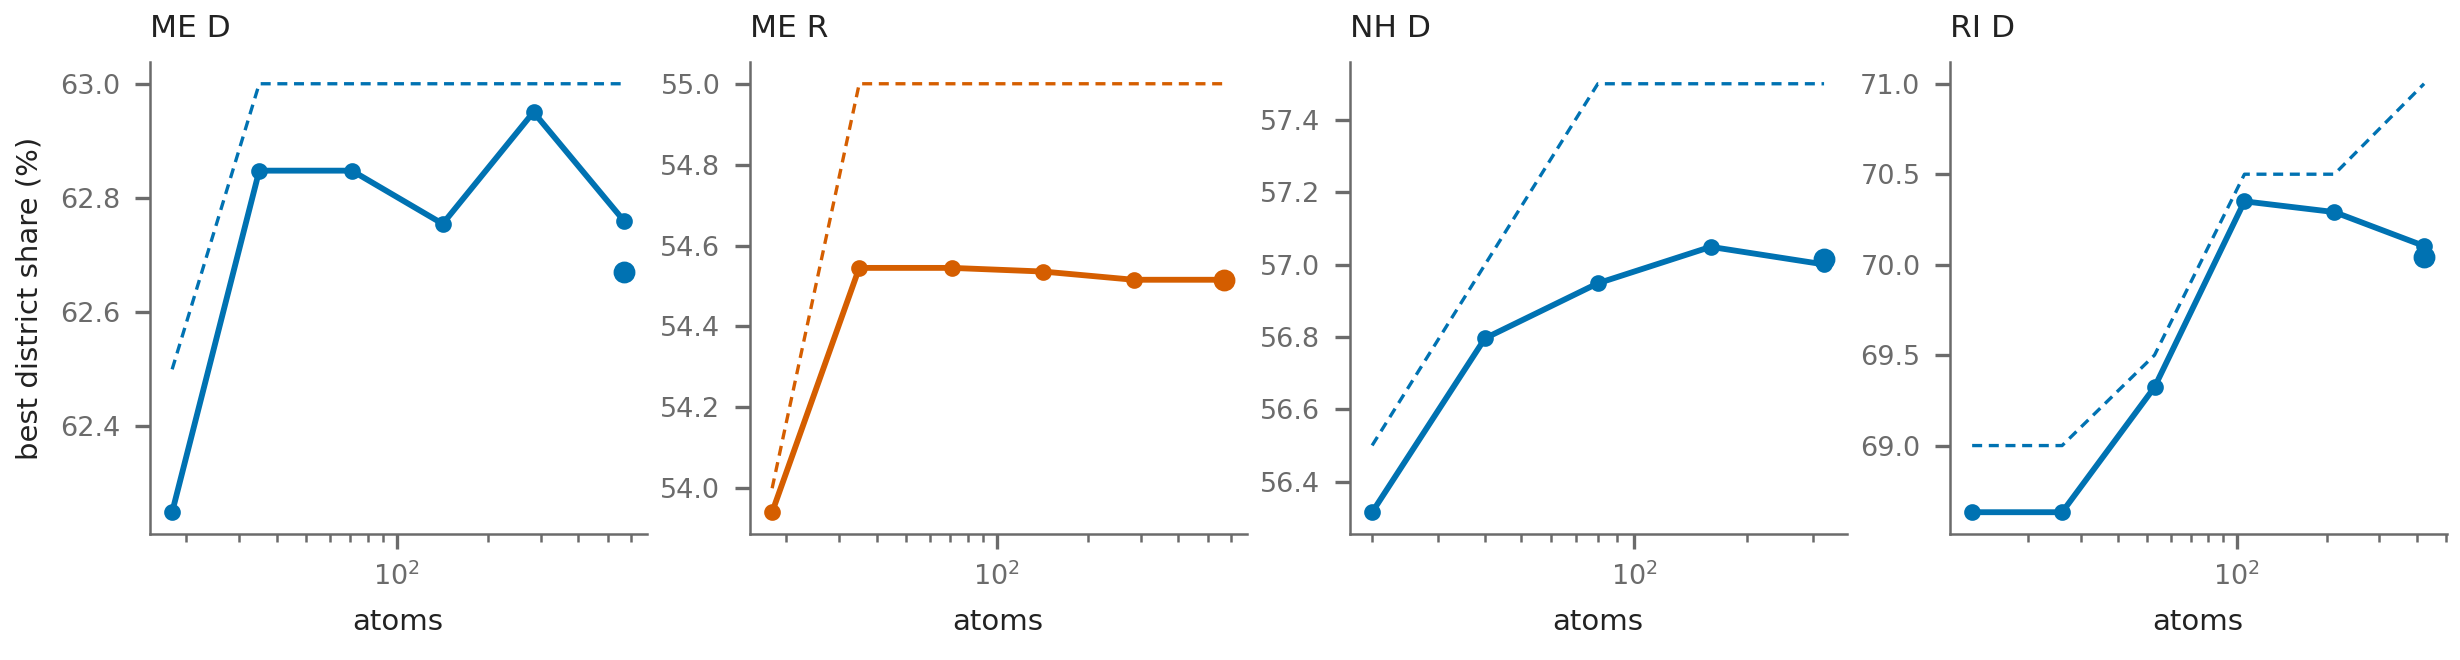
\includegraphics[width=\linewidth]{figs/ladder.png}
\caption{Resolution ladder: best-district share ($q=1$, $s=k-1$) when precincts are merged into fewer, larger atoms (plans keep merged atoms whole, so each rung is a lower-bound class for the next). Solid: best verified plan on the coarse instance; dashed: proven upper end for the coarse instance; large dot: the certified bracket at full precinct resolution. Non-monotone wiggles are heuristic search noise.}\label{fig:ladder}
\end{figure}

\paragraph{Resolution.}
Figure~\ref{fig:ladder} merges precincts, using the same homogeneity hierarchy as the algorithm, into $1/16,\dots,1/2$ as many atoms and recomputes the exact frontier. Because coarser atoms only shrink the plan class, each rung is a lower bound for the next, and the frontier saturates early: with a quarter of the precincts the best-district share is within 0.25 point of its precinct-level value in New Hampshire, Maine (both parties) and Rhode Island Democrats, and with a sixteenth it is within 0.7 point except in Rhode Island (1.5 points). This is evidence about sensitivity to \emph{coarser} atoms only; it does not bound what splitting precincts (or blocks, with an allocation model for the votes) could add.


\subsection{Audits and sanity checks}\label{sec:audit}

Every claim above is a lower bound (a plan) or an upper bound (an infeasibility proof), and each kind was checked separately.

\paragraph{Plans.}
All stored witness plans (514 plan records across the eight run sets) were re-verified from scratch after the runs by the independent verifier of Section~\ref{sec:data}, which recomputes labels, population, connectivity, split counts and every robust margin from raw data with rational arithmetic; none failed, and the exact $q$-th margin recomputed with fractions equals the recorded one. During the runs every plan returned by any solver was verified before it could enter a bracket; this caught one real bug (a cache keyed without the margin, which produced a plan that was not safe) that would otherwise have gone unnoticed.

\paragraph{Proofs.}
(i) \emph{Brute force.} On 72 random toy instances ($3\times4$ to $4\times5$ grids with random populations, votes and county labels, $k=2,3$, tolerance 20\%, budgets $s\in\{\infty,1,2\}$, both parties, several margins) the CEGAR answer for every $q$ equals the exact value from full enumeration of all plans, every relaxation along a random refinement chain is at least the exact value (validity), non-increasing along refinement (Theorem~\ref{thm:mono}), and equal to it at the atomic partition (Theorem~\ref{thm:exact}); none of the 72 failed. The pool relaxations, the safe-first decomposition and the county-aware recombination search pass 22 analogous checks. (ii) \emph{Second solver.} An independently written MILP encoding (single-commodity-flow connectivity, one linear split row, HiGHS with outer-safe tolerances) agrees with CP-SAT on 675 of 675 toy queries over all partitions of the refinement chains, on all 61 stored infeasibility proofs of the six two-district states (each re-derived by the loop and re-checked by HiGHS on the same final partition: 59 agree, 2 remain undecided after 300 s, none disagree), and on 163 of the 203 stored proofs of the states with three to five districts whose final partition is on file (the other 40 are undecided after 120 s; none disagree). An earlier random sample of 116 proofs gave the same picture (103 agree, 13 not re-derivable within the limit, 0 disagree). ``Undecided'' is never counted as agreement. The first version of this audit disagreed with CP-SAT on toy instances with $k=3$ and $s=2$ because the two encodings counted the budget differently (a bug in the audit encoding, not in the CEGAR model); after the fix all queries agree.

\paragraph{Sanity checks.}
(a) The statewide identity: no verified plan has $q=k$ safe districts above the statewide margin, and no proven upper end for $q=1$ lies below it. (b) Party symmetry: the pipeline run on New Hampshire with the two parties' votes exchanged returns the opposite party's brackets ($[57.02,57.5)$ and $[53.74,54.0)$ against $[57.02,57.5)$ and $[53.75,54.0)$). (c) Cross-run consistency: over 104 (state, party, $q$) keys with bounds from up to six independent run sets (and 248 keys across all regimes of Sections~\ref{sec:budget} and~\ref{sec:robust}), every verified lower end is strictly below every proven upper end. (d) Data: state populations equal the Census resident populations, statewide presidential totals reproduce the certified returns, atoms with more votes than residents hold under 0.7\% of the votes in every state. (e) Prior art: the geography-free hull bound, run on Massachusetts (nine districts; 2020 presidential vote, $\pm1\%$; not among our 16 states), allows Republicans at most one district with 50\% or more (best share below 52\%) and no second, in line with the finding of \citet{duchin2019} that Republicans are structurally locked out of district-sized collections of precincts there (their elections differ from ours, so the agreement is qualitative).


\section{Discussion and limitations}\label{sec:disc}

\paragraph{What was learned.}
Certifying the extremes of partisan districting at realistic resolution is possible, but only where the regime supplies structure that a relaxation can exploit. Connectivity is a local property, so a coarse quotient graph cannot see it (Proposition~\ref{prop:blind} and Section~\ref{sec:negative}); the subdivision budget is what turns the county level into an informative abstraction. Counting the budget by \emph{pieces} matters: allowing one county to be cut among all districts for a single ``split'' leaves a large unconstrained sub-problem inside that county and makes the relaxations of the states with $k\ge3$ far looser. With $k=2$ every regime of this type coincides and the loop closes essentially all brackets to half a point of district share; with $k\ge3$ most brackets remain several points wide near the margin at which the relaxation stops being spuriously feasible, and each such query then requires reasoning about the exact boundary of a single district at precinct level, which is the problem the abstraction was meant to avoid. We report those widths rather than tuning the time limits per state.

\paragraph{Reading the numbers.}
$\sigma^*(1)$ minus a party's statewide share measures the ``packing gain'' the boundaries can deliver to that party's single best district; $\sigma^*(k)$ is pinned by the statewide share (the turnout-weighted mean of the district margins equals the statewide margin), and the seats in between interpolate. Because the frontier is a capacity, its exact value at, say, 55\% is a property of the vote geography and the regime, not a forecast: it says nothing about whether any map with that many safe districts would or could be enacted. Both parties are always computed with identical code and, for both, many entries are ``zero'': a party with 39\% statewide (Rhode Island Republicans) provably cannot make a majority district in any plan of the regime.

\paragraph{Limitations.}
\begin{itemize}[leftmargin=*]
\item \emph{Atoms.} The plan class respects precinct boundaries. Splitting precincts enlarges the plan class, so our upper bounds do not bound such plans; the resolution ladder of Section~\ref{sec:robust} indicates how quickly the frontier saturates as atoms are refined, but with observed (not allocated) votes a block-level statement would require an allocation model.
\item \emph{Regime.} A tolerance of $\pm1\%$ and a budget of $k-1$ county splits are modelling choices, not legal standards; the paper makes no legal claim. Compactness, minority-opportunity and other legal constraints are not modelled. They only shrink the plan class, so by Proposition~\ref{prop:mono} our certified upper bounds remain valid upper bounds for any such sub-regime (the lower-bound plans need not satisfy the extra rules). Counties are the subdivisions everywhere, including New England.
\item \emph{Data.} Shares are two-party shares from the 2020 presidential race (robustness variants use every available statewide contest); third parties, turnout changes and other elections are outside the model, and a handful of precincts straddle counties. Island states (Hawaii) are excluded because contiguity across water is ambiguous. Artificial bridge edges (Rhode Island: one; Arkansas: four) are documented in Table~\ref{tab:instances}.
\item \emph{Solvers.} Upper bounds rest on an exact-integer CP-SAT search. We audit them against an independent MILP encoding and brute-force enumeration, but no machine-checkable proof format is produced; certificates are reproducible rather than independently verifiable objects. Lower-bound plans are stored and independently verified.
\item \emph{Coverage.} Only states with $2\le k\le5$ were run (16 states; Hawaii is excluded as above), and time limits (Section~\ref{sec:results}) leave some brackets open. The six single-district states are trivial ($F(m)=1$ exactly when the statewide share is at least $\tfrac12+m$); the 27 states with $k\ge6$ were not attempted, and nothing here says how the method scales to them.
\end{itemize}

\paragraph{Extensions.}
The hierarchy is agnostic to the atom: block-level atoms with an explicit downscaling model, or an outer relaxation over all downscalings, would extend the certificates below the precinct. Additional necessary conditions (compactness measures, opportunity districts) can be added to the relaxation, and the separability of Proposition~\ref{prop:sep} turns state certificates into national ones once the larger states are within reach. The negative result suggests where the algorithmic effort should go: strengthening the relaxation \emph{inside} a split county (for example with connectivity-aware local hulls, which we tried in simple form without gain on New Hampshire) and stronger primal search near the transition margin.

\paragraph{Use.}
The frontier quantifies the mathematical capacity of district boundaries under a stated regime. It is symmetric in the parties, recommends no map and gives no evidence about intent. We hope certified brackets make claims about what is or is not achievable by redistricting easier to check.

\bibliography{refs}
\appendix
\section{Full tables}\label{app:tables}
\begin{table}[h]
\centering\footnotesize
\caption{Upper bounds and incumbents for the share of the most extreme district ($q=1$), in percent of the two-party vote: geography-free hull bound, quotient-connectivity relaxations without budget (counties as cells; after two refinement levels), unconstrained ReCom incumbent, and the certified bracket under $s=k-1$.}\label{tab:ablation}
\begin{tabular}{llcrrrrr}
\toprule
State & Party & $q$ & geo-free & county quot. & refined quot. & ReCom (no budget) & certified, $s{=}k{-}1$ \\
\midrule
New Hampshire & D & 1 & 62.4 & 62.5 & 63.0 & 57.0 & 57.02--57.5 \\
New Hampshire & R & 1 & 54.6 & 55.0 & 55.0 & -- & $<$50 \\
Maine & D & 1 & 66.7 & 67.0 & 67.0 & 63.3 & 62.67--63.0 \\
Maine & R & 1 & 57.9 & 58.0 & 58.0 & 54.8 & 54.52--55.0 \\
Rhode Island & D & 1 & 72.4 & 73.0 & 72.5 & 69.6 & 70.04--70.5 \\
Rhode Island & R & 1 & 50.0 & 50.0 & 50.0 & -- & $<$50 \\
Idaho & D & 1 & 50.0 & 50.0 & 50.0 & -- & $<$50 \\
Idaho & R & 1 & 79.6 & 80.0 & 80.0 & 74.5 & 75.50--76.0 \\
Montana & D & 1 & 57.3 & 57.5 & 57.5 & -- & 50.00--52.5 \\
Montana & R & 1 & 72.9 & 73.0 & 73.0 & 66.6 & 67.53--69.5 \\
West Virginia & D & 1 & 50.0 & 50.0 & 50.0 & -- & $<$50 \\
West Virginia & R & 1 & 80.4 & 80.5 & 80.5 & 74.0 & 76.00--77.0 \\
Nebraska & D & 1 & 63.2 & 63.5 & 63.5 & 58.6 & 58.63--61.5 \\
Nebraska & R & 1 & 79.6 & 80.0 & 80.0 & 78.4 & 78.31--79.0 \\
New Mexico & D & 1 & 76.6 & 77.0 & 77.0 & 69.2 & 69.28--74.0 \\
New Mexico & R & 1 & 68.0 & 68.5 & 68.5 & 59.6 & 60.98--66.5 \\
Arkansas & D & 1 & 70.7 & 71.5 & 71.0 & 54.5 & 55.60--62.5 \\
Arkansas & R & 1 & 84.9 & 85.5 & 85.0 & 78.8 & 79.86--81.5 \\
Iowa & D & 1 & 67.9 & 68.0 & 68.0 & 60.1 & 61.37--64.5 \\
Iowa & R & 1 & 72.9 & 73.5 & 73.0 & 68.7 & 68.80--71.0 \\
Kansas & D & 1 & 68.8 & 69.5 & 69.5 & 60.5 & 60.85--65.0 \\
Kansas & R & 1 & 80.2 & 81.0 & 81.0 & 75.2 & 75.84--78.5 \\
Mississippi & D & 1 & 83.7 & 84.5 & 84.0 & 63.7 & 65.79--70.0 \\
Mississippi & R & 1 & 87.6 & 88.0 & 88.0 & 71.4 & 72.26--80.0 \\
Nevada & D & 1 & 71.4 & 72.0 & 72.0 & 67.5 & 67.86--70.5 \\
Nevada & R & 1 & 65.6 & 66.0 & 66.0 & 55.8 & 55.91--64.0 \\
Utah & D & 1 & 67.4 & 68.0 & 68.0 & 64.5 & 64.77--66.5 \\
Utah & R & 1 & 81.9 & 82.5 & 82.5 & 77.5 & 78.19--81.0 \\
Connecticut & D & 1 & 82.7 & 83.0 & 83.5 & 71.1 & 70.12--82.5 \\
Connecticut & R & 1 & 55.0 & 55.5 & 55.0 & 50.7 & 50.03--55.0 \\
Oklahoma & D & 1 & 65.8 & 66.5 & 66.0 & 53.4 & 54.19--63.5 \\
Oklahoma & R & 1 & 85.3 & 86.0 & 85.5 & 81.9 & 81.70--83.5 \\
\bottomrule
\end{tabular}

\end{table}

{\footnotesize\begin{longtable}{llccccc}
\caption{Certified brackets $[r_q,u_q)$ for $\sigma^*(q)$ in percent of the two-party vote ($50\%+m$), merged over all runs and including the geography-free upper bound. ``$<$50'' means $\sigma^*(q)<0$ is proved (fewer than $q$ districts can reach 50\%). $^\dagger$: bracket wider than 0.5 point.}\label{tab:spectrum} \\
\toprule
State & Party & $q=1$ & $q=2$ & $q=3$ & $q=4$ & $q=5$ \\
\midrule
\endfirsthead
\toprule
State & Party & $q=1$ & $q=2$ & $q=3$ & $q=4$ & $q=5$ \\
\midrule
\endhead
New Hampshire & D & [57.02, 57.5) & [53.75, 53.8) &  &  &  \\
New Hampshire & R & $<$50 & $<$50 &  &  &  \\
Maine & D & [62.67, 63.0) & [54.62, 54.7) &  &  &  \\
Maine & R & [54.52, 55.0) & $<$50 &  &  &  \\
Rhode Island & D & [70.04, 70.5) & [60.60, 60.6) &  &  &  \\
Rhode Island & R & $<$50 & $<$50 &  &  &  \\
Idaho & D & $<$50 & $<$50 &  &  &  \\
Idaho & R & [75.50, 76.0) & [65.88, 65.9) &  &  &  \\
Montana & D & [50.00, 52.5)$^\dagger$ & $<$50 &  &  &  \\
Montana & R & [67.53, 69.5)$^\dagger$ & [58.40, 58.4) &  &  &  \\
West Virginia & D & $<$50 & $<$50 &  &  &  \\
West Virginia & R & [76.00, 77.0)$^\dagger$ & [69.78, 69.8) &  &  &  \\
Nebraska & D & [58.63, 61.5)$^\dagger$ & [49.68, 51.5)$^\dagger$ & $<$50 &  &  \\
Nebraska & R & [78.31, 79.0)$^\dagger$ & [66.85, 69.5)$^\dagger$ & [59.71, 59.8) &  &  \\
New Mexico & D & [69.28, 74.0)$^\dagger$ & [62.35, 65.0)$^\dagger$ & [55.21, 55.6) &  &  \\
New Mexico & R & [60.98, 66.5)$^\dagger$ & [51.08, 54.5)$^\dagger$ & $<$50 &  &  \\
Arkansas & D & [55.60, 62.5)$^\dagger$ & [42.38, 54.5)$^\dagger$ & $<$50 & $<$50 &  \\
Arkansas & R & [79.86, 81.5)$^\dagger$ & [74.36, 79.5)$^\dagger$ & [69.94, 73.5)$^\dagger$ & [64.13, 64.3) &  \\
Iowa & D & [61.37, 64.5)$^\dagger$ & [55.15, 59.5)$^\dagger$ & [50.29, 52.9)$^\dagger$ & $<$50 &  \\
Iowa & R & [68.80, 71.0)$^\dagger$ & [64.20, 66.5)$^\dagger$ & [57.51, 60.9)$^\dagger$ & [54.02, 54.2) &  \\
Kansas & D & [60.85, 65.0)$^\dagger$ & [52.19, 58.0)$^\dagger$ & [46.10, 51.0)$^\dagger$ & $<$50 &  \\
Kansas & R & [75.84, 78.5)$^\dagger$ & [67.86, 72.7)$^\dagger$ & [64.06, 65.5)$^\dagger$ & [51.80, 57.5)$^\dagger$ &  \\
Mississippi & D & [65.79, 70.0)$^\dagger$ & [52.31, 66.0)$^\dagger$ & [44.96, 53.0)$^\dagger$ & $<$50 &  \\
Mississippi & R & [72.26, 80.0)$^\dagger$ & [69.45, 79.0)$^\dagger$ & [65.67, 70.5)$^\dagger$ & [57.44, 58.4)$^\dagger$ &  \\
Nevada & D & [67.86, 70.5)$^\dagger$ & [60.36, 64.0)$^\dagger$ & [54.06, 55.0)$^\dagger$ & [47.20, 51.3)$^\dagger$ &  \\
Nevada & R & [55.91, 64.0)$^\dagger$ & [55.49, 57.0)$^\dagger$ & [50.60, 53.0)$^\dagger$ & $<$50 &  \\
Utah & D & [64.77, 66.5)$^\dagger$ & [51.95, 54.0)$^\dagger$ & $<$50 & $<$50 &  \\
Utah & R & [78.19, 81.0)$^\dagger$ & [73.20, 75.0)$^\dagger$ & [68.15, 70.0)$^\dagger$ & [58.82, 60.7)$^\dagger$ &  \\
Connecticut & D & [70.12, 82.5)$^\dagger$ & [67.98, 73.5)$^\dagger$ & [64.27, 67.5)$^\dagger$ & [60.81, 64.0)$^\dagger$ & [60.12, 60.2) \\
Connecticut & R & [50.03, 55.0)$^\dagger$ & $<$50 & $<$50 & $<$50 & $<$50 \\
Oklahoma & D & [54.19, 63.5)$^\dagger$ & [43.92, 53.0)$^\dagger$ & $<$50 & $<$50 & $<$50 \\
Oklahoma & R & [81.70, 83.5)$^\dagger$ & [78.30, 81.0)$^\dagger$ & [75.27, 77.9)$^\dagger$ & [70.85, 73.7)$^\dagger$ & [66.52, 67.0) \\
\bottomrule
\end{longtable}
}
\end{document}
